\documentclass[11pt]{article}
\usepackage{fullpage}
\usepackage{graphicx}
\usepackage{longtable}
\usepackage{booktabs}
\usepackage{hyperref}

\providecommand{\tightlist}{%
  \setlength{\itemsep}{0pt}\setlength{\parskip}{0pt}}

\title{Design}
\date{}

\setlength\LTleft{0pt}
\setlength\LTright{0pt}

\setlength{\parskip}{\baselineskip}%
\setlength{\parindent}{0pt}%

\begin{document}
\maketitle
\tableofcontents
\newpage

\section{High-Level}\label{high-level}

The high-level design serves as a transition between the requirements
and the full low-level design. Below are designs used to identify key
components of the system and how they shall interact, both with each
other and with the user.

\subsection{Context Model}\label{context-model}

As with many computer games, this system is mostly `self-enclosed' -
that is, it does not require a large amount of interaction with
separately-developed external systems. Thus, the context of the Ant Game
system is minimal. However, unlike many other computer games, the style
of the game can require the user to provide some external `data' before
playing (an ant brain, and sometimes an ant-world). This means that
there is a possibility for external programs to be developed to aid the
user in writing a custom ant brain/world. This would mean that there
would be an interaction between the Ant Game program and two other
systems, as below:

\begin{center}
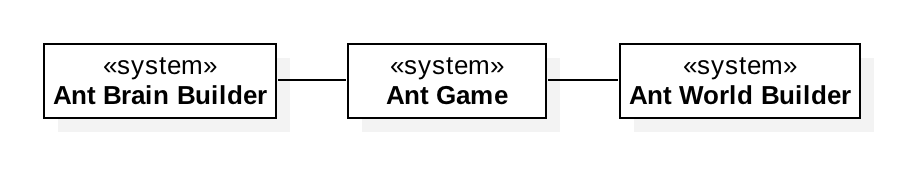
\includegraphics{high-level-diagrams/context-model.png}
\end{center}

However, as per the functional requirements document (\texttt{Game/4}
and \texttt{World/1}) the program shall parse ant brains and worlds from
a \emph{file} (i.e.~only indirectly received from outside software), so
this interaction with external programs does not need to be accounted
for in development.

\subsection{Process Model}\label{process-model}

\subsubsection{User Process}\label{user-process}

The process model on the following page describes a player interacting with the ant game
system. Note that the only two actions where the user is not directly
interacting with the program is the \texttt{Build\ Ant\ Brain} action
and \texttt{Build\ World} action - both of these actions are done
independently of this system by the user (in a text editor or
otherwise). This process model is abstract enough that it applies to
both the two-player game and the tournament. It is assumed that at least
two users are following this process model at the same time, and
interacting with the same instance of the program.

\begin{center}
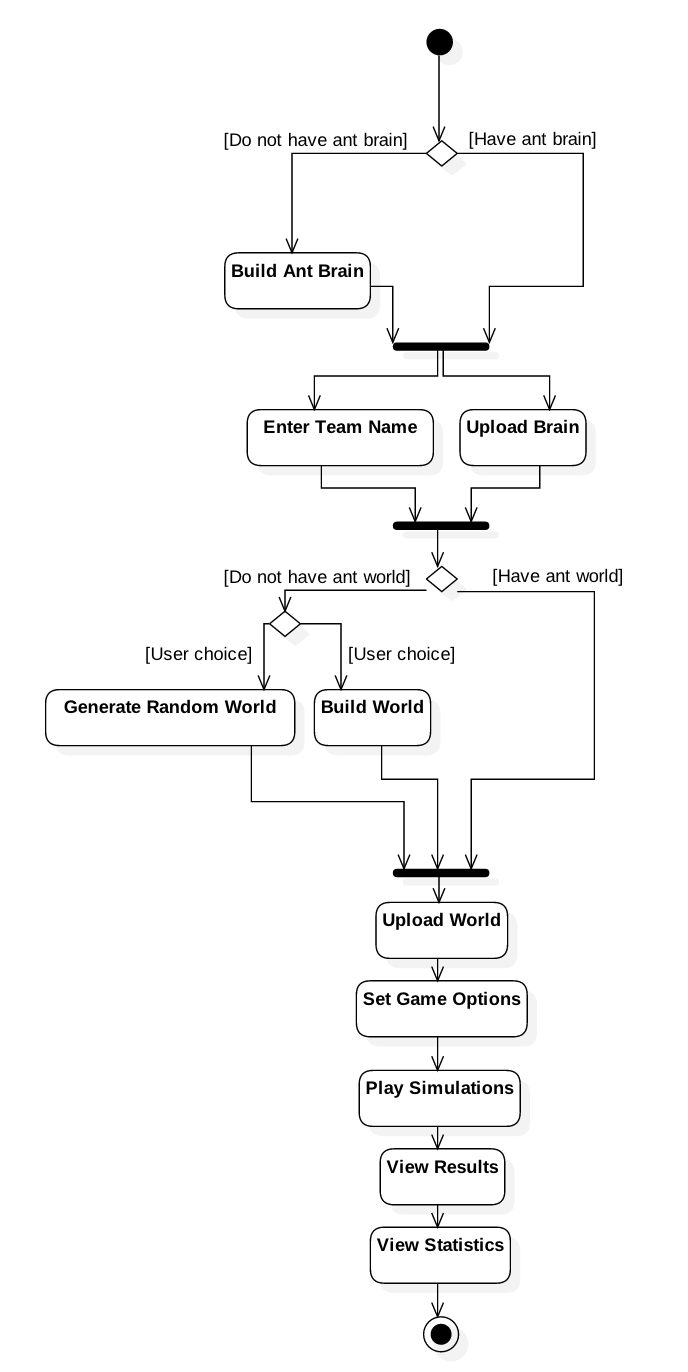
\includegraphics[width=\textwidth,height=\textheight,keepaspectratio]{high-level-diagrams/process-model.png}
\end{center}

\subsubsection{Game Process}\label{game-process}

The following diagram gives a high-level view of the flow of the system
when simulating a game between two ant colonies on a particular world.
Ant brains and a single world are loaded by two actors (the players).
The system then initialises ants on the two anthills for each colony.
Each ants identifiers are also initialised, as per the order in the
functional requirements. The game is then started, lasting for 300,000
rounds. Once the round counter is at its maximum, the food at each
anthill is counted; the team with the most food at their brains anthill
is declared the winner.

\begin{center}
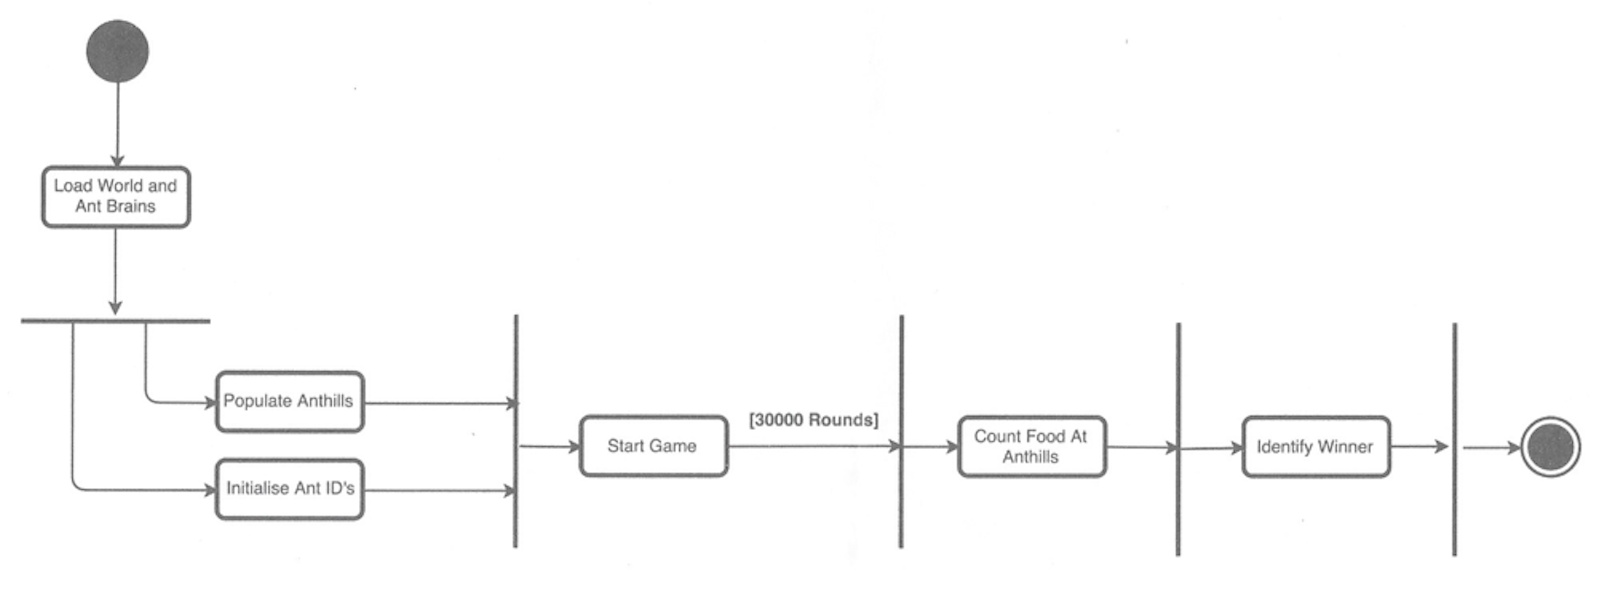
\includegraphics[width=\textwidth]{high-level-diagrams/process-model-game.png}
\end{center}

\subsection{Use Cases}\label{use-cases}

The process model makes it clearer as to how the user will interact with
the system. From the process model and the requirements, the primary use
cases of the system have been extracted, as below. The only (human)
actors in the following use cases are the players of the game.

\subsubsection{Upload Ant Brain}\label{upload-ant-brain}

\begin{center}
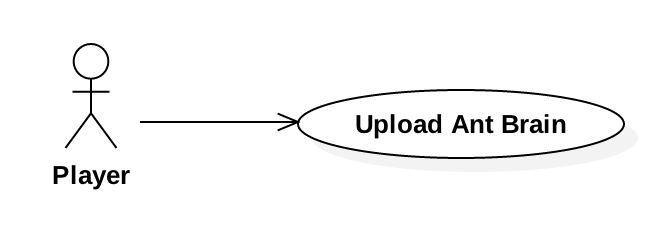
\includegraphics[width=0.4\textwidth]{high-level-diagrams/use-case-1-upload-ant-brain.png}
\end{center}

\begin{longtable}[c]{@{}p{0.2\textwidth}p{0.7\textwidth}@{}}
\toprule
& Ant Game: Upload Ant Brain\tabularnewline
\midrule

Actors & Each player in a two-player game or a tournament. That is,
although not interacting with each user simultaneously, the system will
be interacting with multiple users in turn.\tabularnewline
Description & In order to simulate a game, the players must upload their
custom ant brains. These must be parsed from file into
memory.\tabularnewline
Data & The location of a file on disk.\tabularnewline
Stimulus & Triggered by user clicking on a file-chooser button,
navigating to the path of the file, and clicking `Parse' (on the game
setup screen of the system's interface).\tabularnewline
Response & Whether the file represented a valid ant brain as per the
functional requirements for parsing given in
\texttt{Parsing\ Specifications/Brain}. If invalid, the system should
inform the user of what went wrong and on which line (if
relevant).\tabularnewline
\bottomrule
\end{longtable}

\subsubsection{Generate Random World}\label{generate-random-world}

\begin{center}
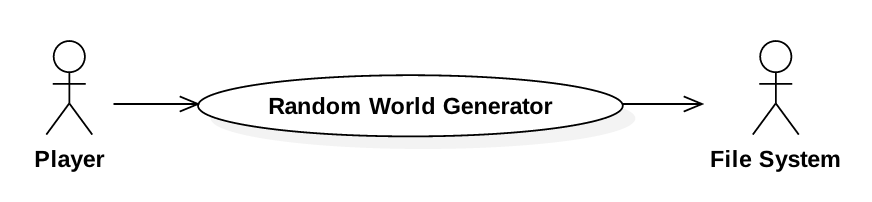
\includegraphics[width=0.4\textwidth]{high-level-diagrams/use-case-2-generate-random-world.png}
\end{center}

\begin{longtable}[c]{@{}p{0.2\textwidth}p{0.7\textwidth}@{}}
\toprule
& Ant Game: Generate Random World\tabularnewline
\midrule

Actors & A player, before a game or tournament.
Filesystem.\tabularnewline
Description & A tournament requires a world that conforms to the
specifications laid out in the functional requirements (see requirement
\texttt{World/2}). This component of the system can be interacted with
by the user to write a random world to file which conforms to these
specifications.\tabularnewline
Data & -\tabularnewline
Stimulus & Triggered by the user by interacting with the GUI, selecting
the option to generate a random ant world.\tabularnewline
Response & Generates a random ant world. Converts the ant world to a
textual description, as per functional requirement
\texttt{Parsing\ Specifications/World}. Asks the user where to save to
on disk, and then writes to a text file at that location.\tabularnewline
\bottomrule
\end{longtable}

\subsubsection{Upload Ant World}\label{upload-ant-world}

\begin{center}
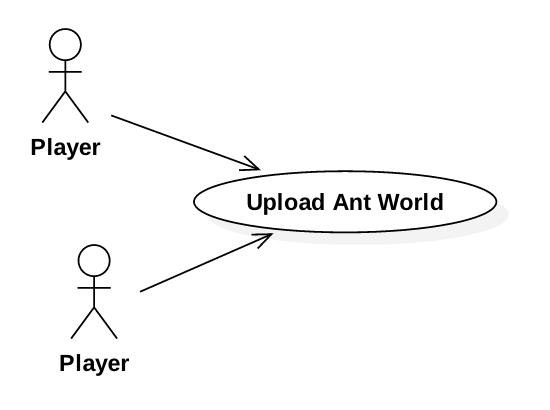
\includegraphics[width=0.4\textwidth]{high-level-diagrams/use-case-3-upload-ant-world.png}
\end{center}

\begin{longtable}[c]{@{}p{0.2\textwidth}p{0.7\textwidth}@{}}
\toprule
& Ant Game: Upload Ant World\tabularnewline
\midrule

Actors & Two or more players who agree to upload a particular ant world
to compete on.\tabularnewline
Description & In order to simulate a game or tournament, there must be
at least one ant world for the ants to compete on. These must be parsed
from file into memory.\tabularnewline
Data & The location of a file on disk.\tabularnewline
Stimulus & On the game and tournament setup screens, there will be a
button to upload an ant world. Once the user clicks on this, chooses a
file to parse, and clicks `Parse', this use case will be
invoked.\tabularnewline
Response & Whether the file represented a valid ant world as per the
functional requirements for parsing given in
\texttt{Parsing\ Specifications/World}. In addition, if this use case is
invoked in the context of a tournament setup, the additional criteria
for a contest world shall be checked (see requirement
\texttt{World/2}).\tabularnewline
\bottomrule
\end{longtable}

\subsubsection{Simulate Two Player Game}\label{simulate-two-player-game}

\begin{center}
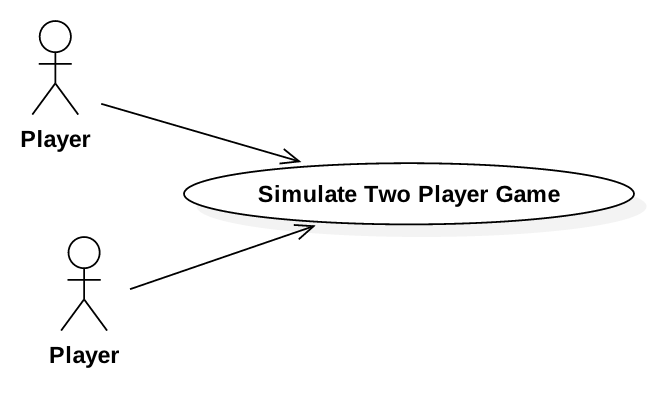
\includegraphics[width=0.4\textwidth]{high-level-diagrams/use-case-4-two-player-game.png}
\end{center}

\begin{longtable}[c]{@{}p{0.2\textwidth}p{0.7\textwidth}@{}}
\toprule
& Ant Game: Simulate Two Player Game\tabularnewline
\midrule

Actors & Two players.\tabularnewline
Description & Once the game setup is complete (with players setting the
ant brains and ant world) this use case comes next, with a competition
between the ants on the world being simulated.\tabularnewline
Data & The contextual data from other use cases will be in memory - the
world and brains. Some other relevant data shall be provided by the
user, such as the team names and options for game viewing (detailed in
the interface design section).\tabularnewline
Stimulus & The `Play' button on the game setup screen.\tabularnewline
Response & The system will simulate a game between the two ant colonies
as described in the functional requirements (\texttt{Game/1}). It will
present a simulation of the world as the ants carry out their actions.
At the end of the simulation, it will display the winner of the game to
the players, as well as relevant game statistics.\tabularnewline
\bottomrule
\end{longtable}

\subsubsection{Tournament}\label{tournament}

\begin{center}
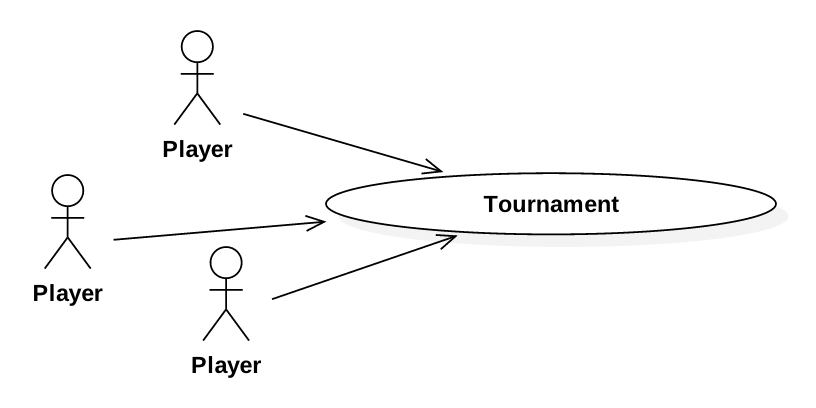
\includegraphics[width=0.4\textwidth]{high-level-diagrams/use-case-5-tournament.png}
\end{center}

\begin{longtable}[c]{@{}p{0.2\textwidth}p{0.7\textwidth}@{}}
\toprule
& Ant Game: Tournament\tabularnewline
\midrule

Actors & Two or more players.\tabularnewline
Description & This use case can be considered a `superset' of the use
Two Player Game use case. Once each of the players have uploaded the ant
brains and ant worlds, they can start a tournament to compete amongst
multiple ant brains on multiple ant worlds, to see which player is the
overall winner.\tabularnewline
Data & The contextual data from other use cases will be in memory - the
worlds (at least one, possibly several) and brains. As above, some other
relevant data shall be provided by the user, such as the team names and
options for game viewing.\tabularnewline
Stimulus & The `Play' button on the tournament setup
screen.\tabularnewline
Response & The system simulates an ant game between every possible
combination of teams, worlds, and colours (red or black). Then it
returns the final results of the tournament to the user (as per the
functional requirement \texttt{Game/3}) as well as statistics on the
game.\tabularnewline
\bottomrule
\end{longtable}

\subsection{System Components}\label{system-components}

From the functional requirements, the process model and use cases, the
main system components and their interactions have been modelled below. Note also the multiplicity between the components.

\begin{center}
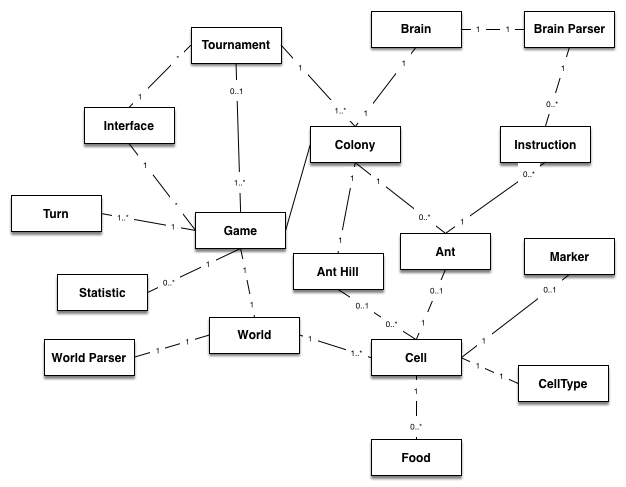
\includegraphics[width=\textwidth]{high-level-diagrams/system-components.png}
\end{center}

The system components diagram is extremely useful in terms of developing
a full design, and is the fundamental building block of the low-level
design section.

\newpage
\section{Low-Level}

The low-level section of the design goes into further detail of how the system is to be implemented. The lower level design has been done is a slightly non-conventional order --- instead of beginning from the system component diagram to develop detailed class diagrams, the initial point of the low-level design has started from the use cases to construct detailed sequence diagrams. From the sequence diagrams, class diagrams have been constructed to validate the design.

\subsection{Sequence Diagrams}

The following sequence diagrams detail, in particular, the behaviour of an ant as it interacts with the world in a game simulation. A single `operation' is described in each sequence, and clearly exposes the relevant components and behaviours associated with the operation. 

\subsubsection{Ant - Drop}

This sequence diagram describes the actions of an ant when performing a \textit{drop} instruction.

\begin{center}
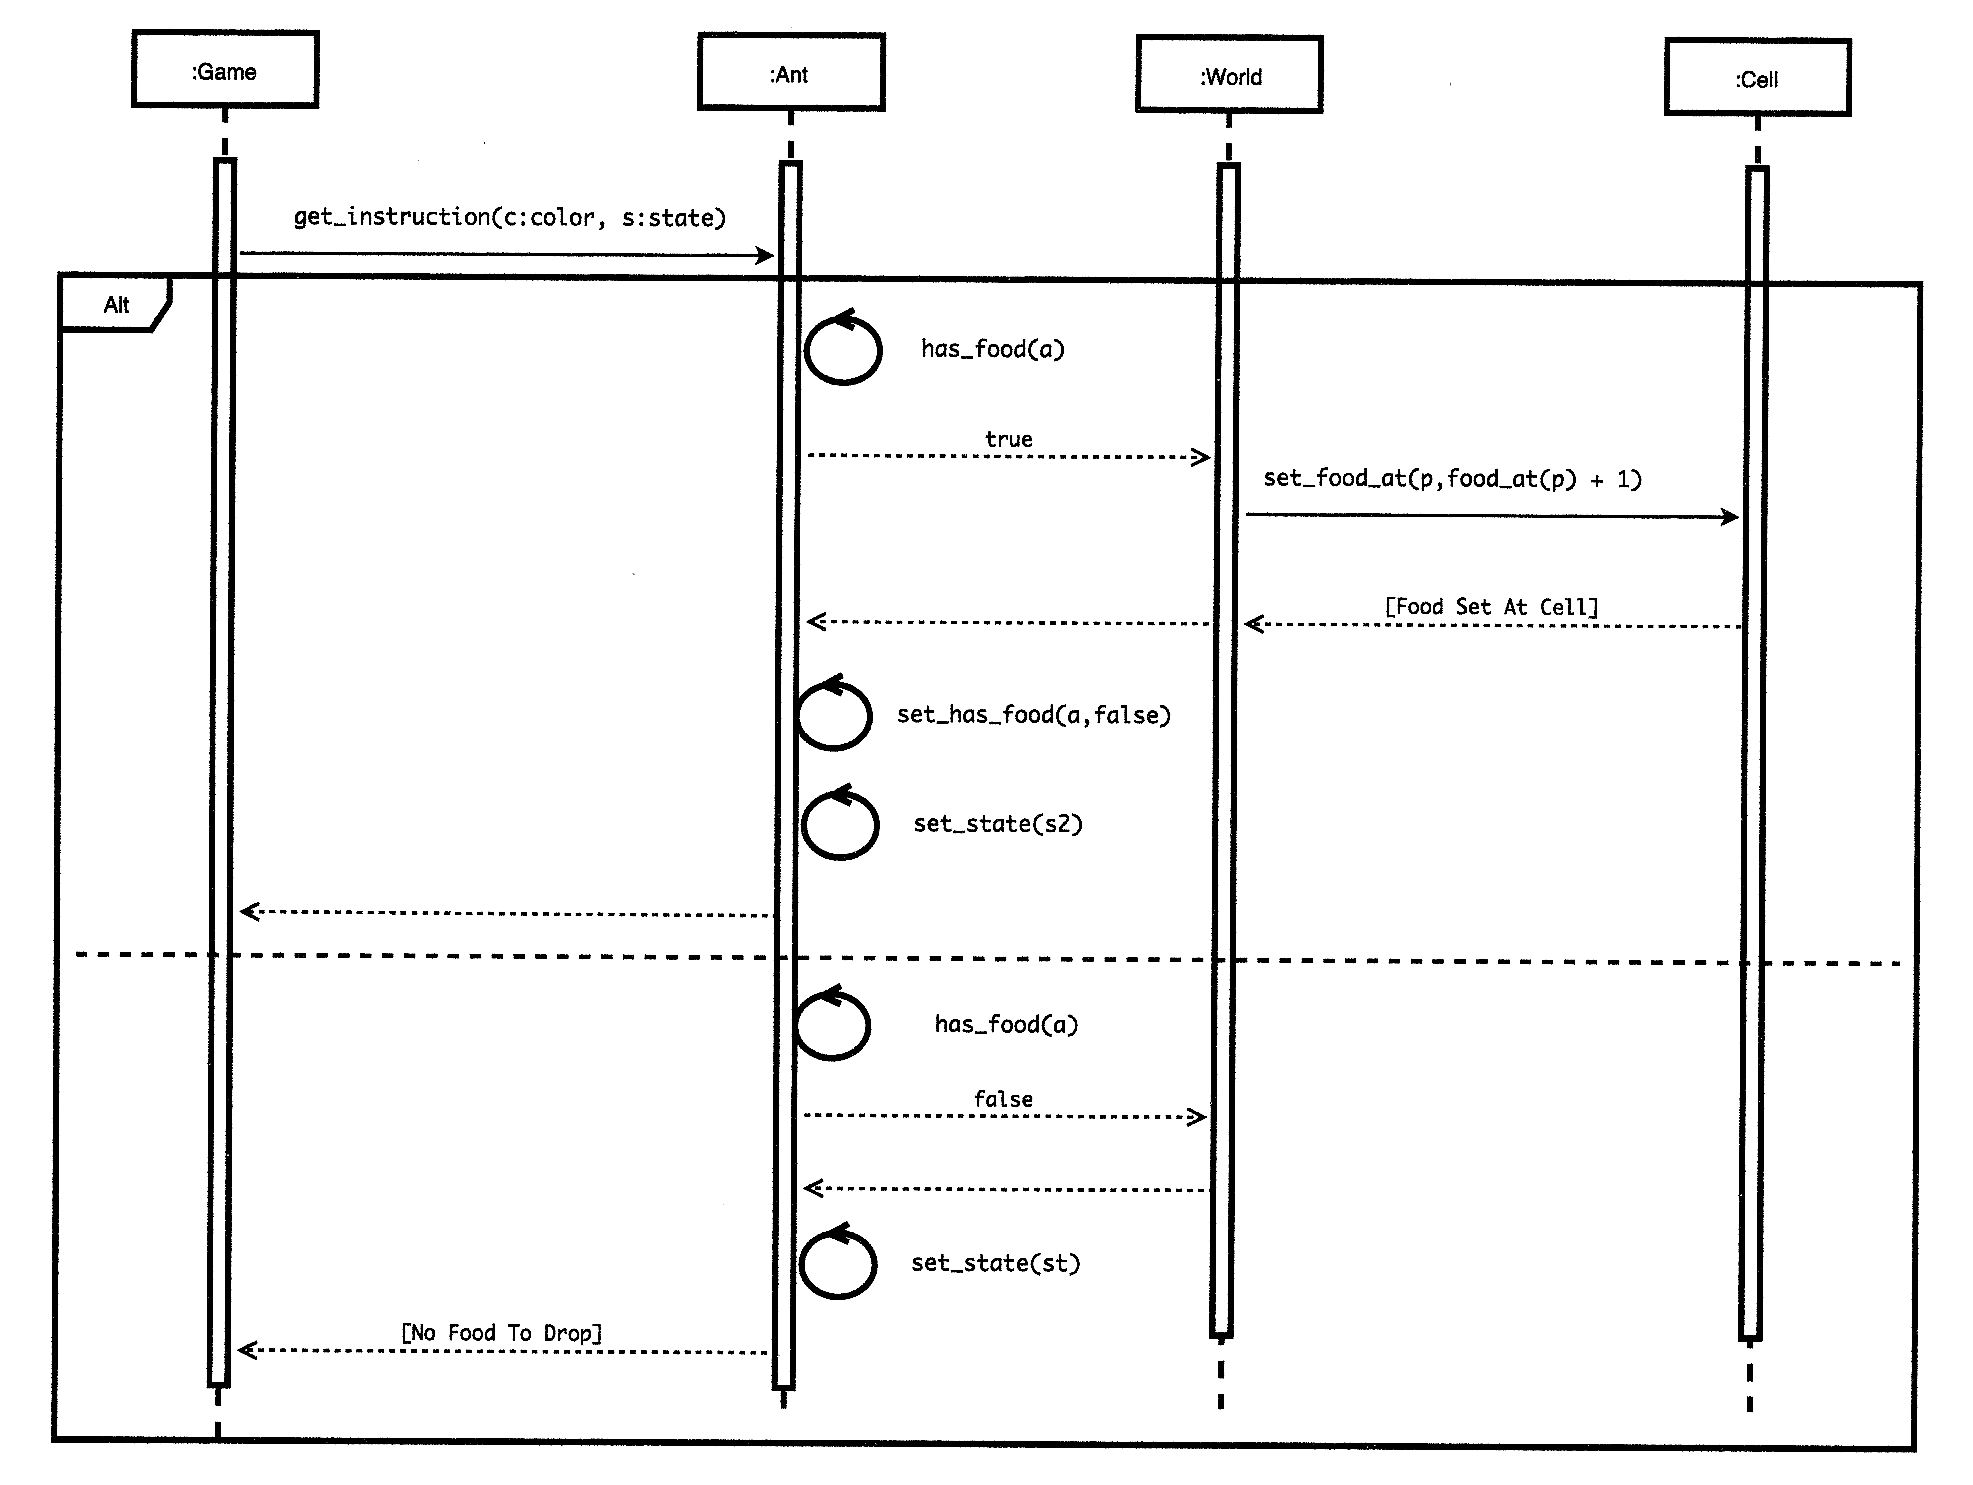
\includegraphics[width=0.8\textwidth]{low-level-diagrams/sequence/ant-drop.png}
\end{center}

\subsubsection{Ant - Flip}

This sequence diagram describes the actions of an ant when performing a \textit{flip} instruction.

\begin{center}
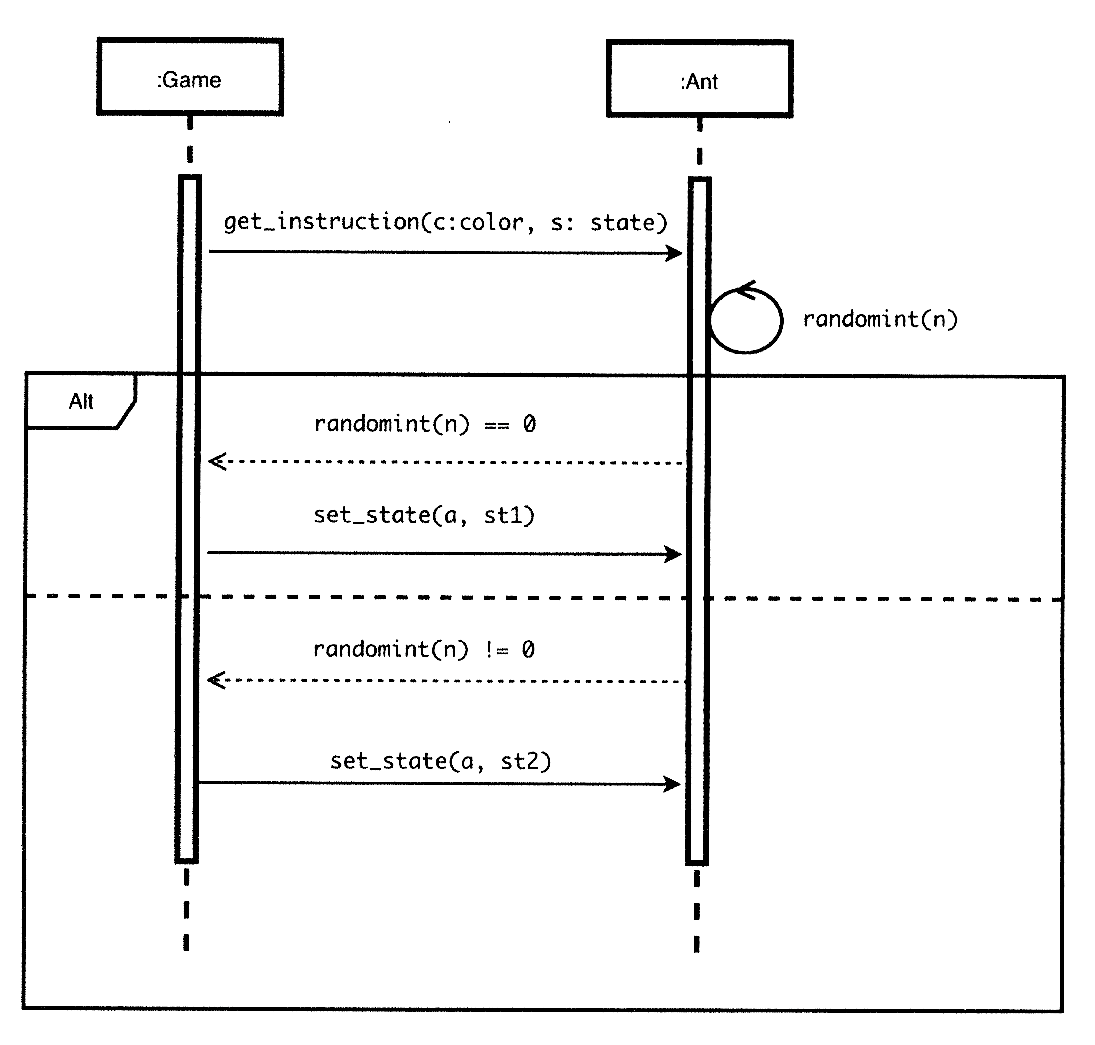
\includegraphics[width=0.8\textwidth]{low-level-diagrams/sequence/ant-flip.png}
\end{center}

\subsubsection{Ant - Mark}

This sequence diagram describes the actions of an ant when performing a \textit{mark} instruction.

\begin{center}
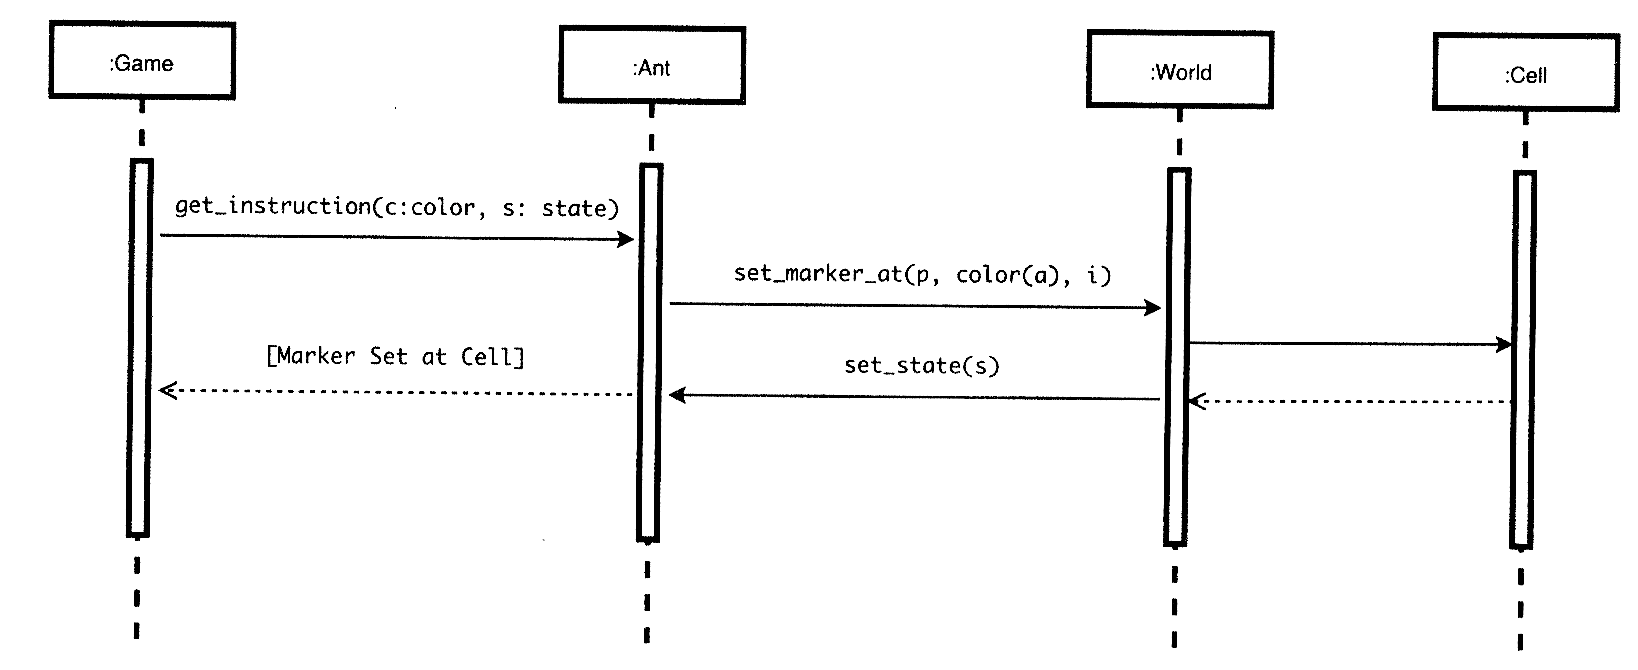
\includegraphics[width=0.8\textwidth]{low-level-diagrams/sequence/ant-mark.png}
\end{center}

\subsubsection{Ant - Move}

This sequence diagram describes the actions of an ant when performing a \textit{move} instruction.

\begin{center}
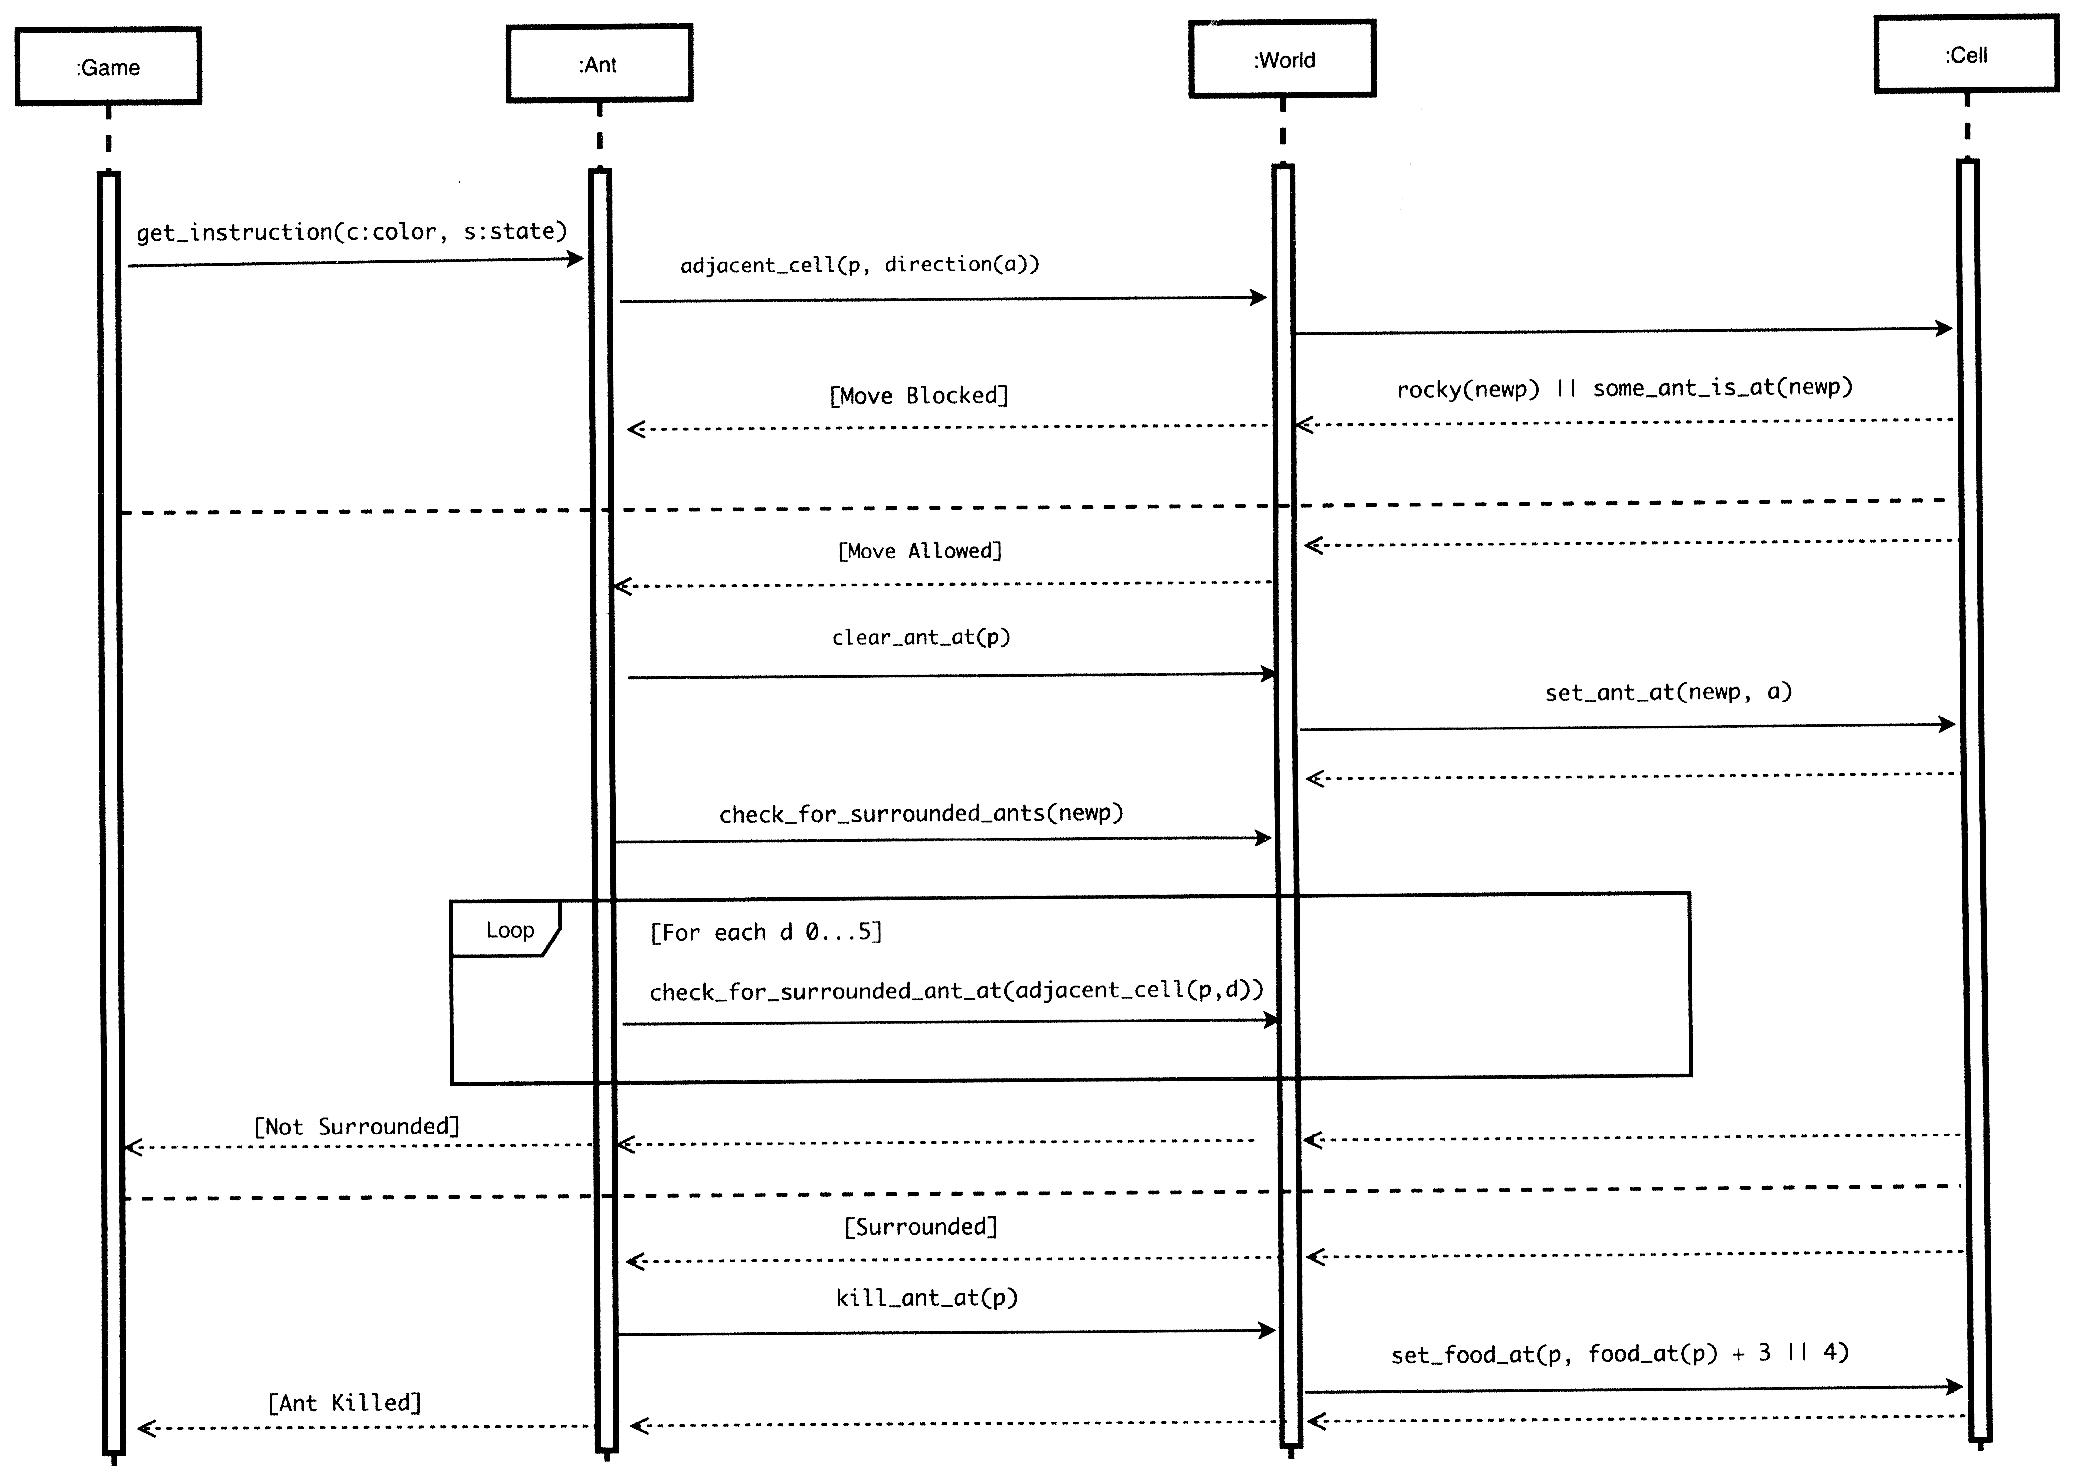
\includegraphics[width=0.8\textwidth]{low-level-diagrams/sequence/ant-move.png}
\end{center}

\subsubsection{Ant - Pick-Up}

This sequence diagram describes the actions of an ant when performing a \textit{pick-up} instruction.

\begin{center}
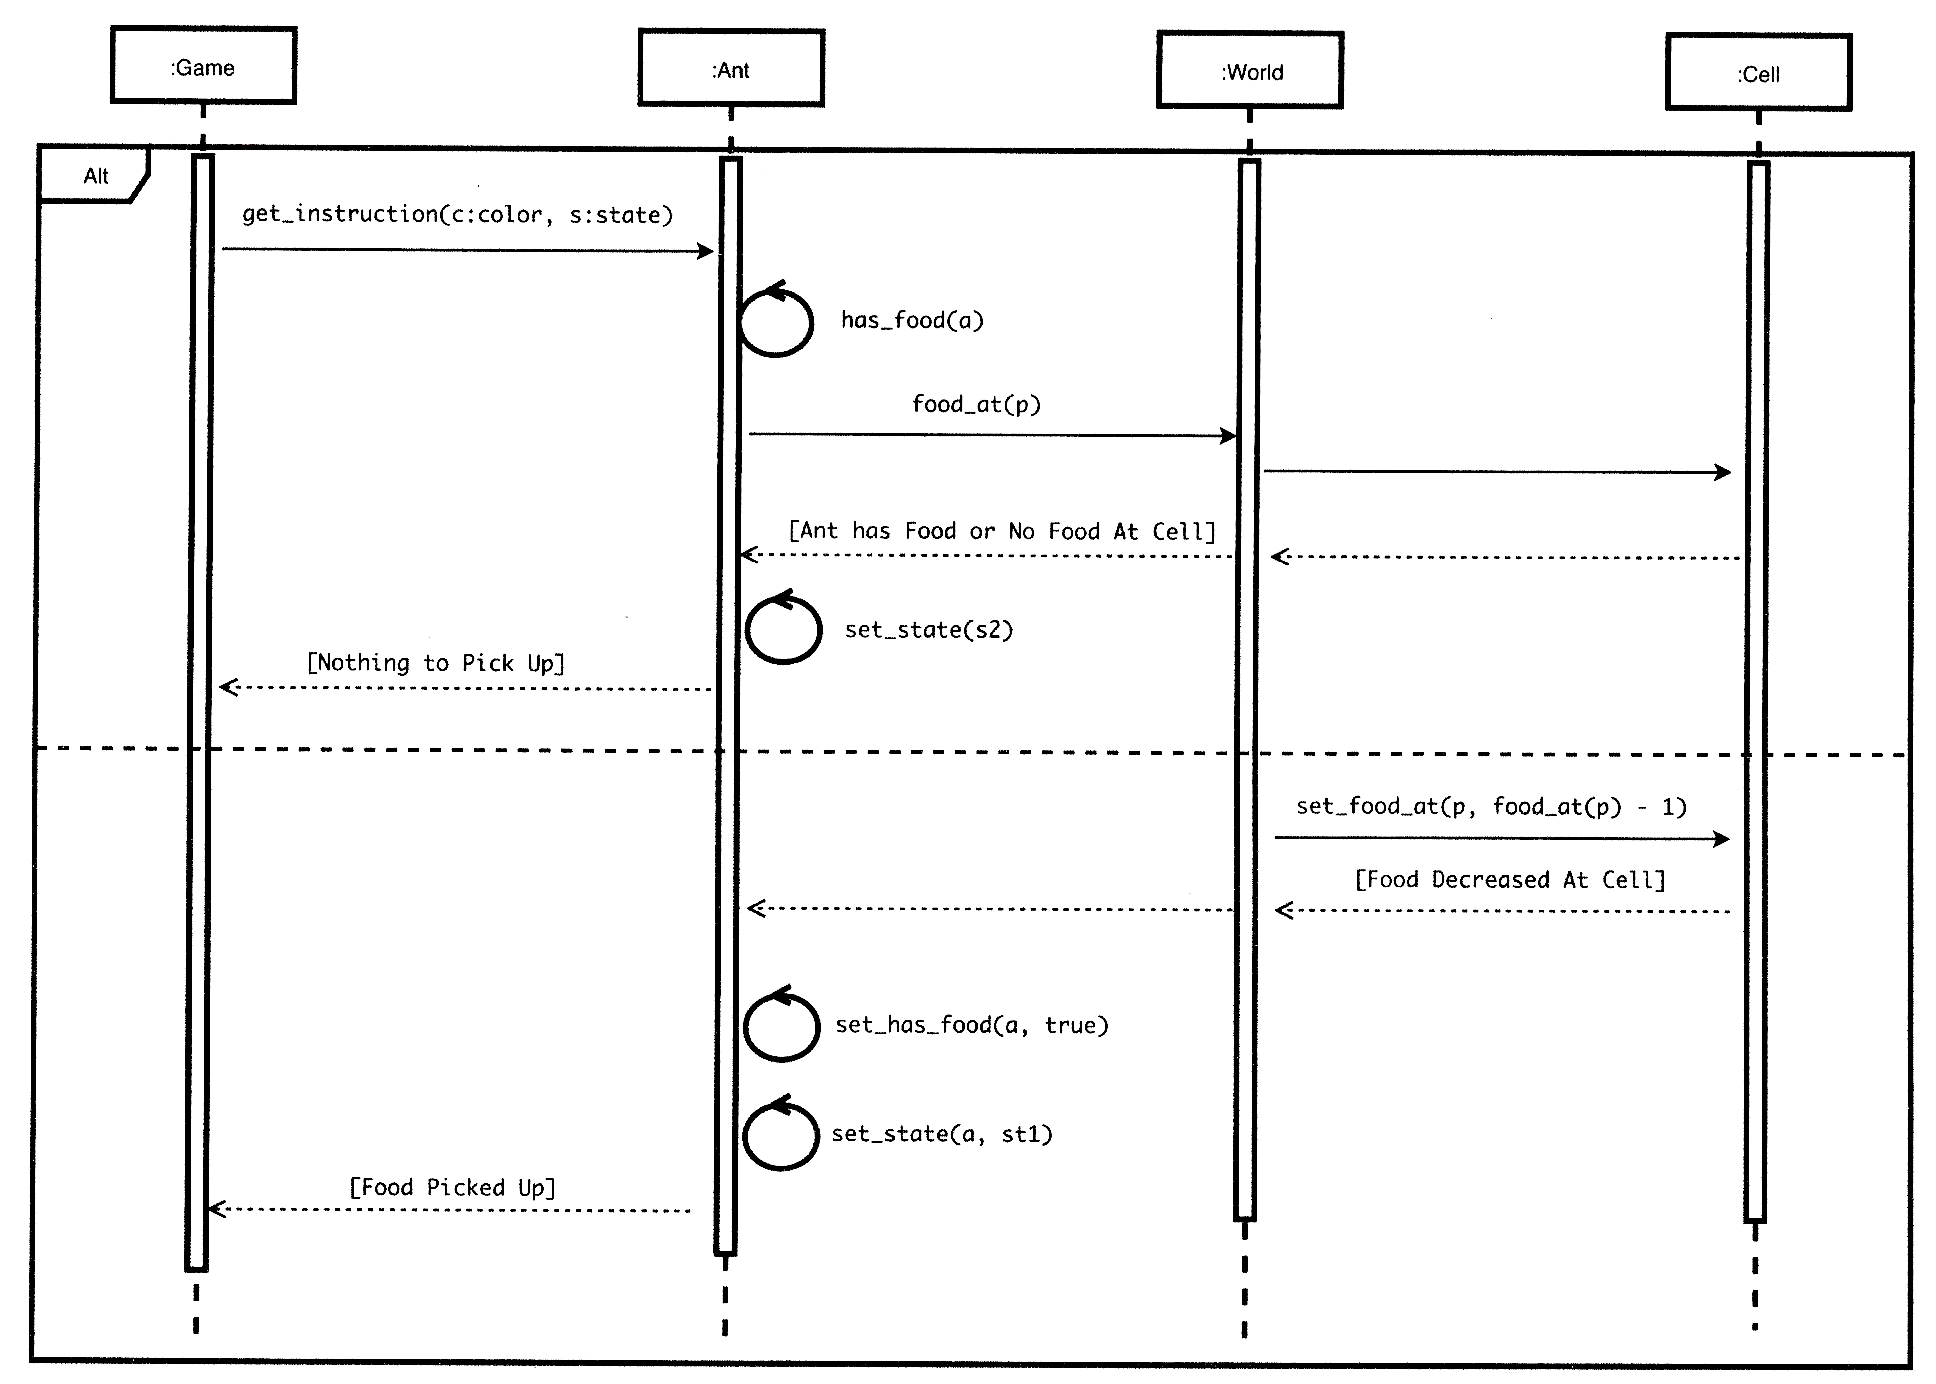
\includegraphics[width=0.8\textwidth]{low-level-diagrams/sequence/ant-pickup.png}
\end{center}

\subsubsection{Ant - Sense}

This sequence diagram describes the actions of an ant when performing a \textit{sense} instruction.

\begin{center}
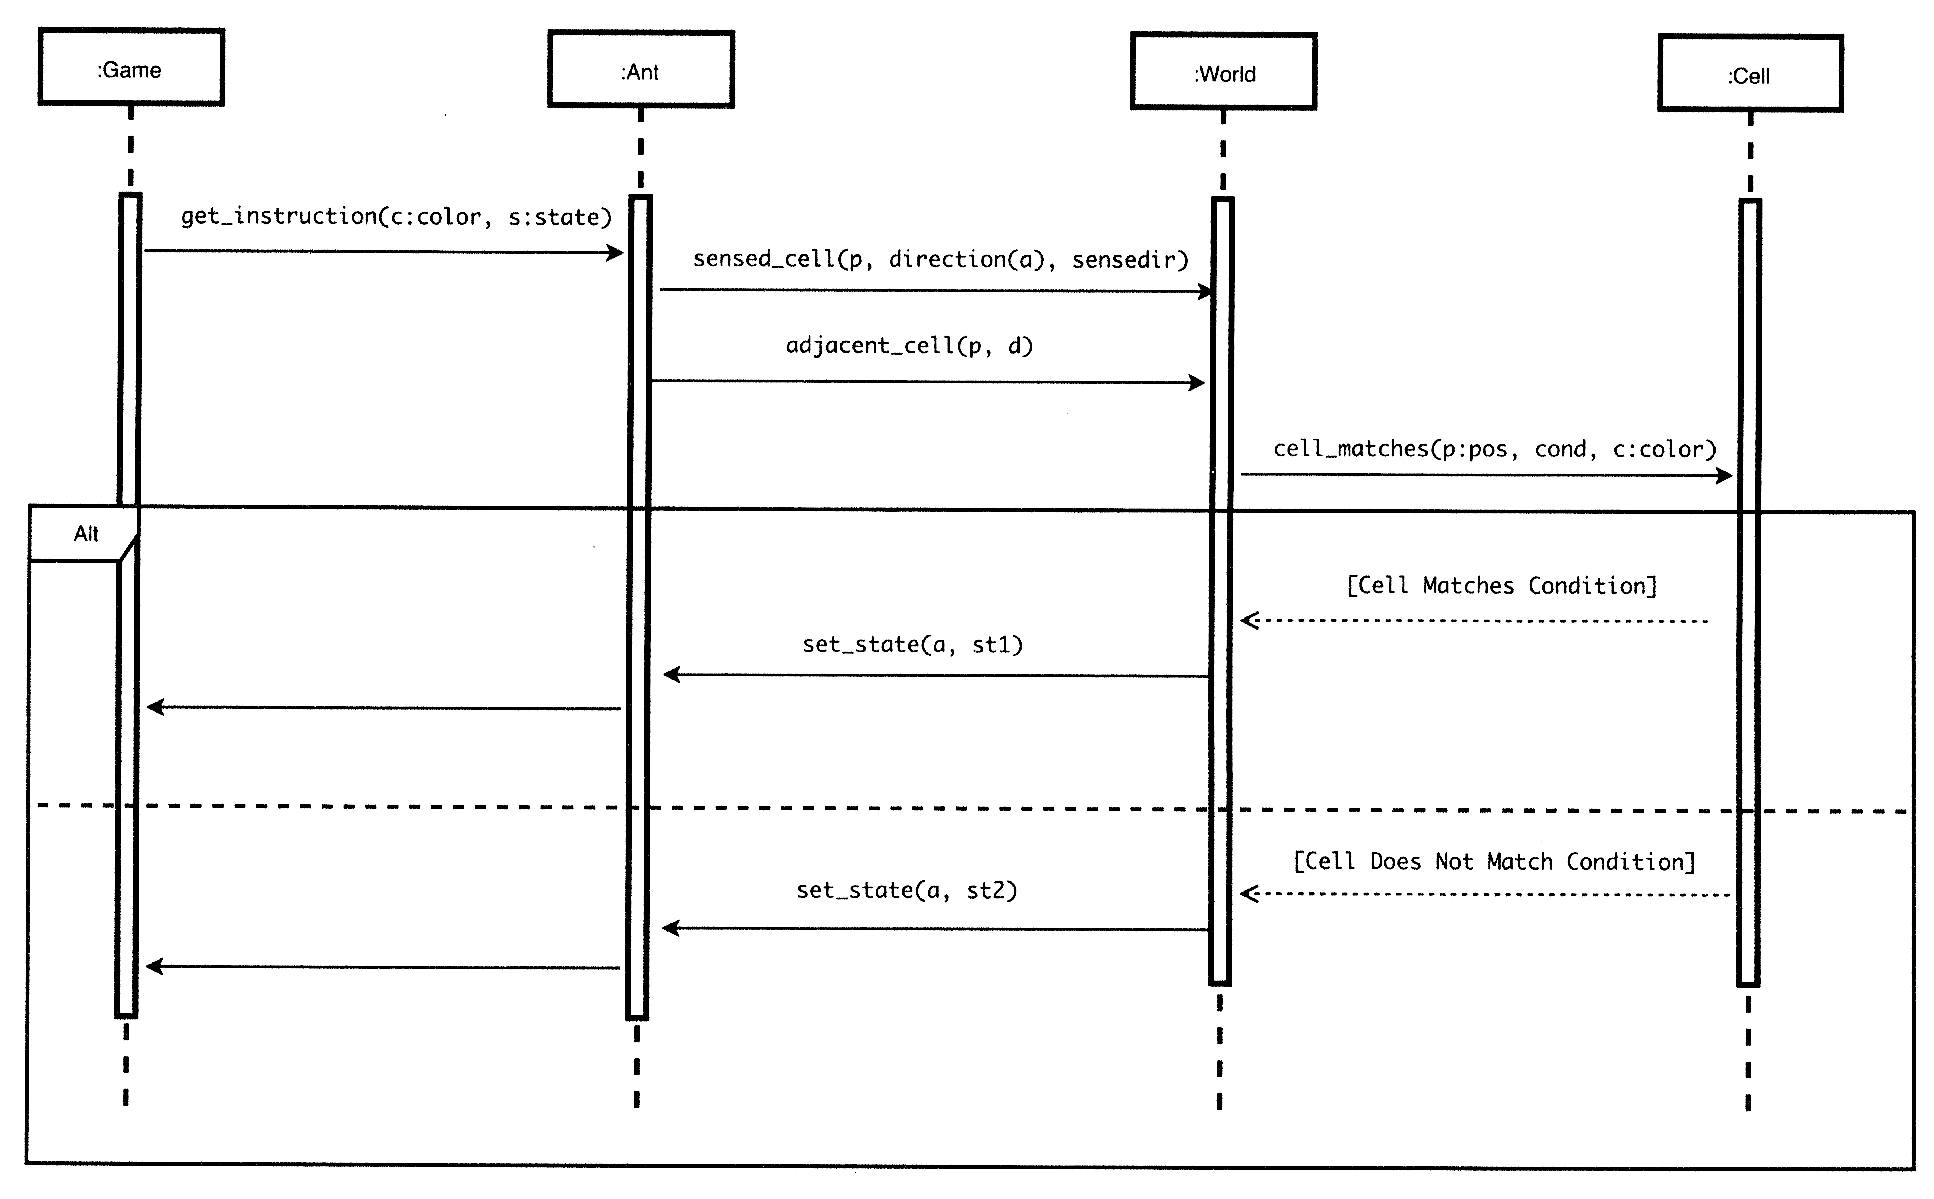
\includegraphics[width=0.8\textwidth]{low-level-diagrams/sequence/ant-sense.png}
\end{center}

\subsubsection{Ant - Turn}

This sequence diagram describes the actions of an ant when performing a \textit{turn} instruction.

\begin{center}
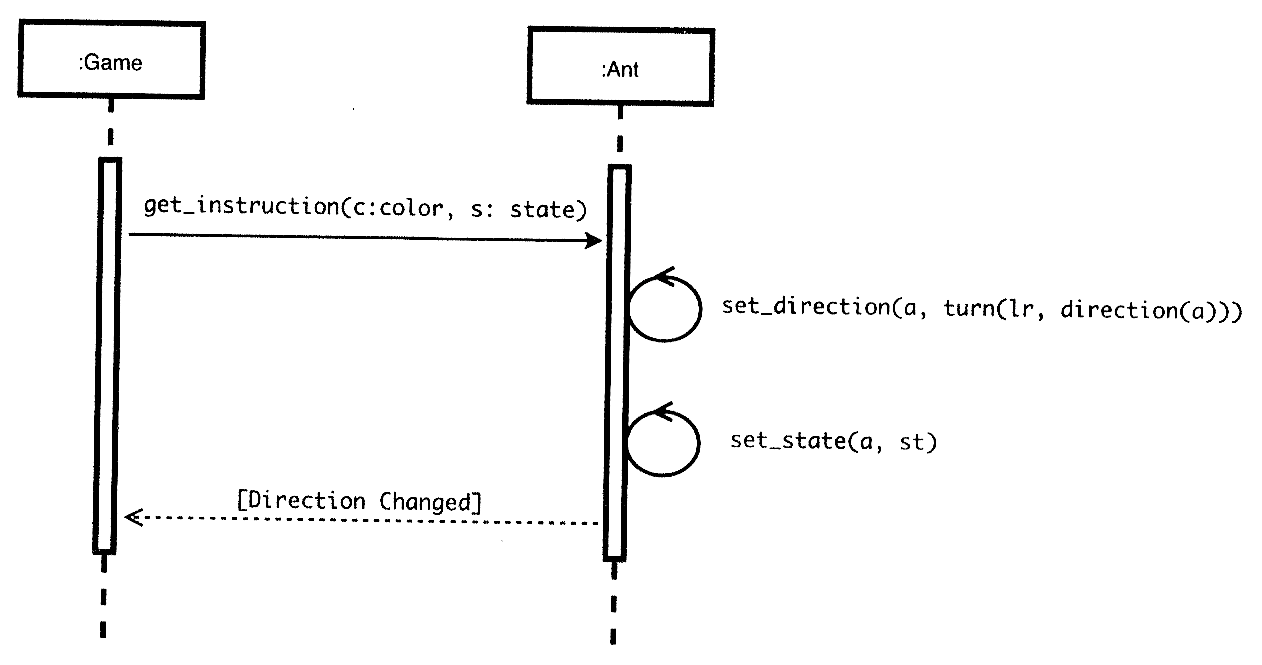
\includegraphics[width=0.8\textwidth]{low-level-diagrams/sequence/ant-turn.png}
\end{center}

\subsubsection{Ant - Unmark}

This sequence diagram describes the actions of an ant when performing an \textit{unmark} instruction.

\begin{center}
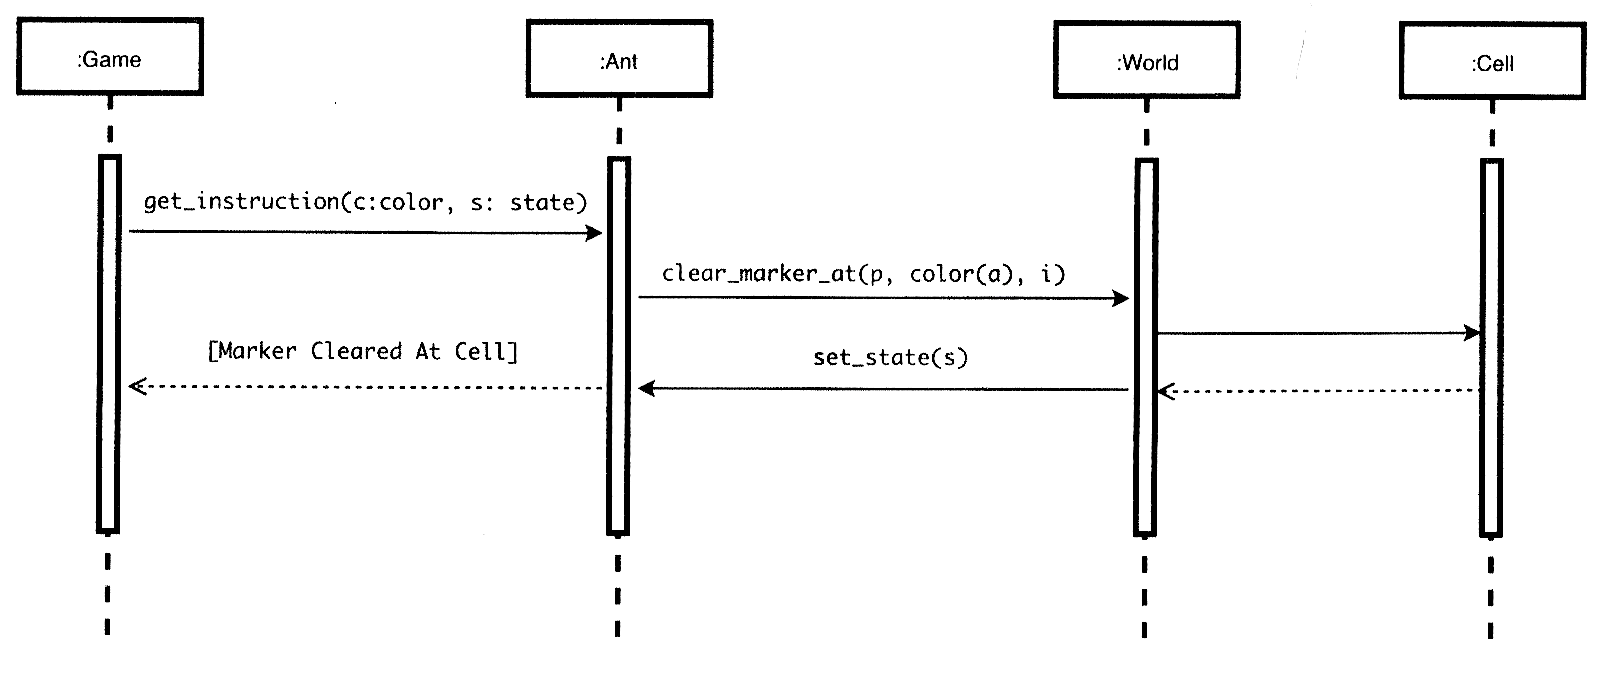
\includegraphics[width=0.8\textwidth]{low-level-diagrams/sequence/ant-unmark.png}
\end{center}

\subsubsection{World - Execute Instruction}

This sequence diagram describes the actions of the world when interacting with the ant to execute an instruction.

\begin{center}
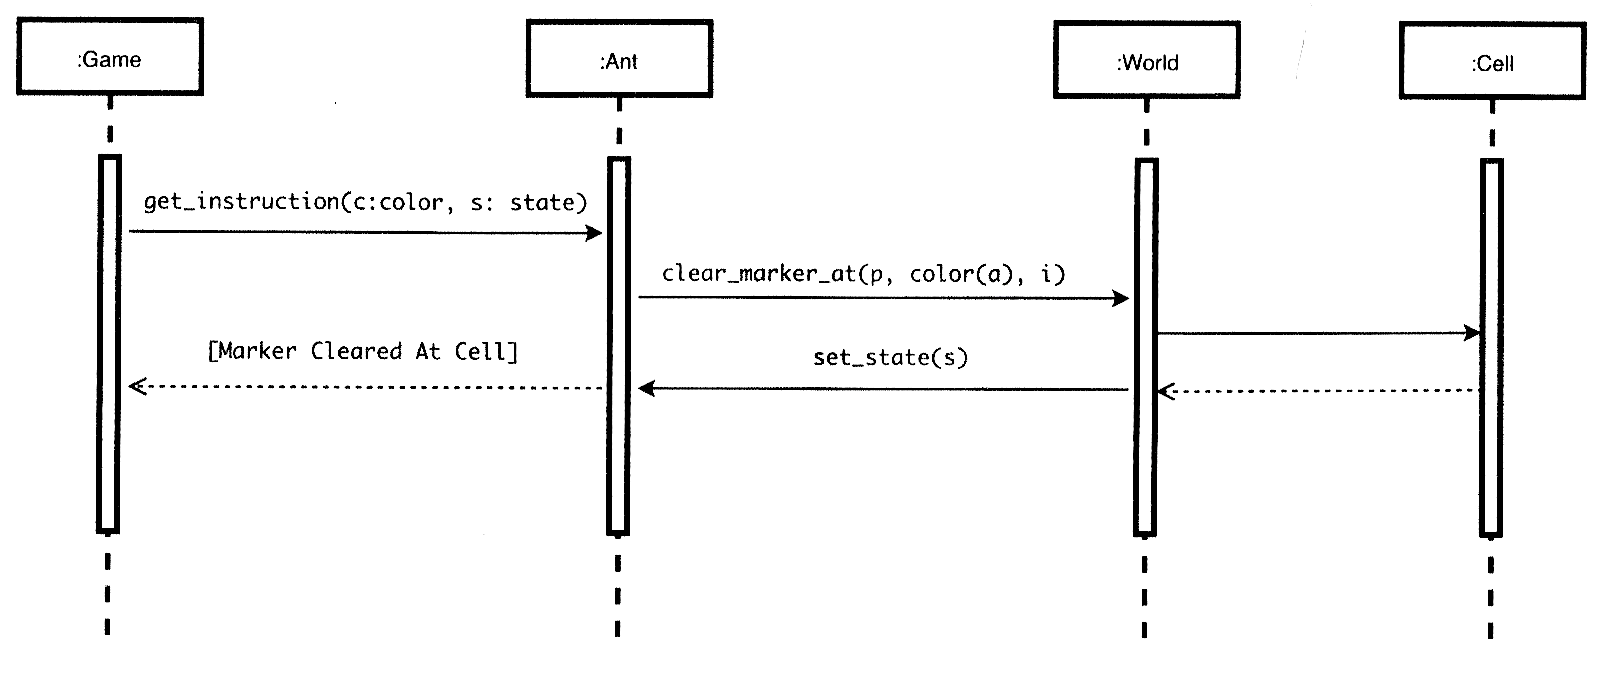
\includegraphics[width=0.8\textwidth]{low-level-diagrams/sequence/ant-unmark.png}
\end{center}

\subsection{Class Diagrams}

The below diagram is an overview of the components which are described in much more detail in this section. Each of the components below is a `module of functionality'. The classes inside each module are highly related, whereas the interaction between the classes of separate modules have minimal coupling.

\begin{center}
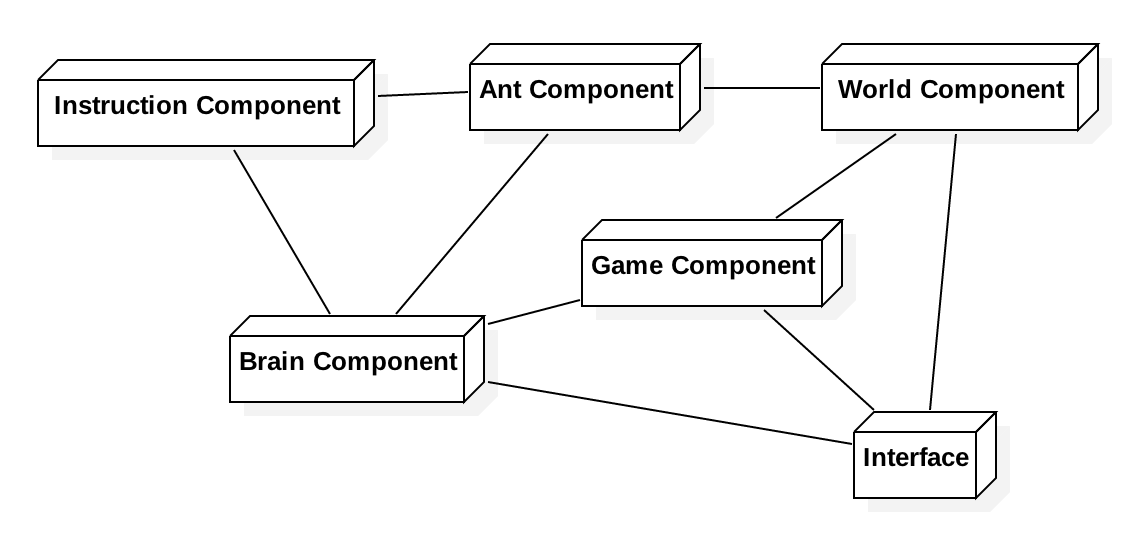
\includegraphics[width=0.8\textwidth]{low-level-diagrams/class/components.png}
\end{center}

The class diagrams in this section have omitted getters and setters for brevity. After each diagram is a brief description of the purpose of each class involved.



\subsubsection{Instructions}

The following diagram abstracts the different type of \textit{instructions} that an ant brain can carry out. This component of the system follows a linked-list style paradigm - an \texttt{Instruction} has two self-referential attributes \texttt{success} and \texttt{failure}, which are the states that the ant brain will transition to depending on whether the ant's action was a success or a failure. Observe that the majority of classes below have little to no operations, only attributes --- this is because the majority of state changes will be handled by other components, whereas this component is primarily for holding data. All classes are immutable, apart from setting the transition instructions.
 
\begin{center}
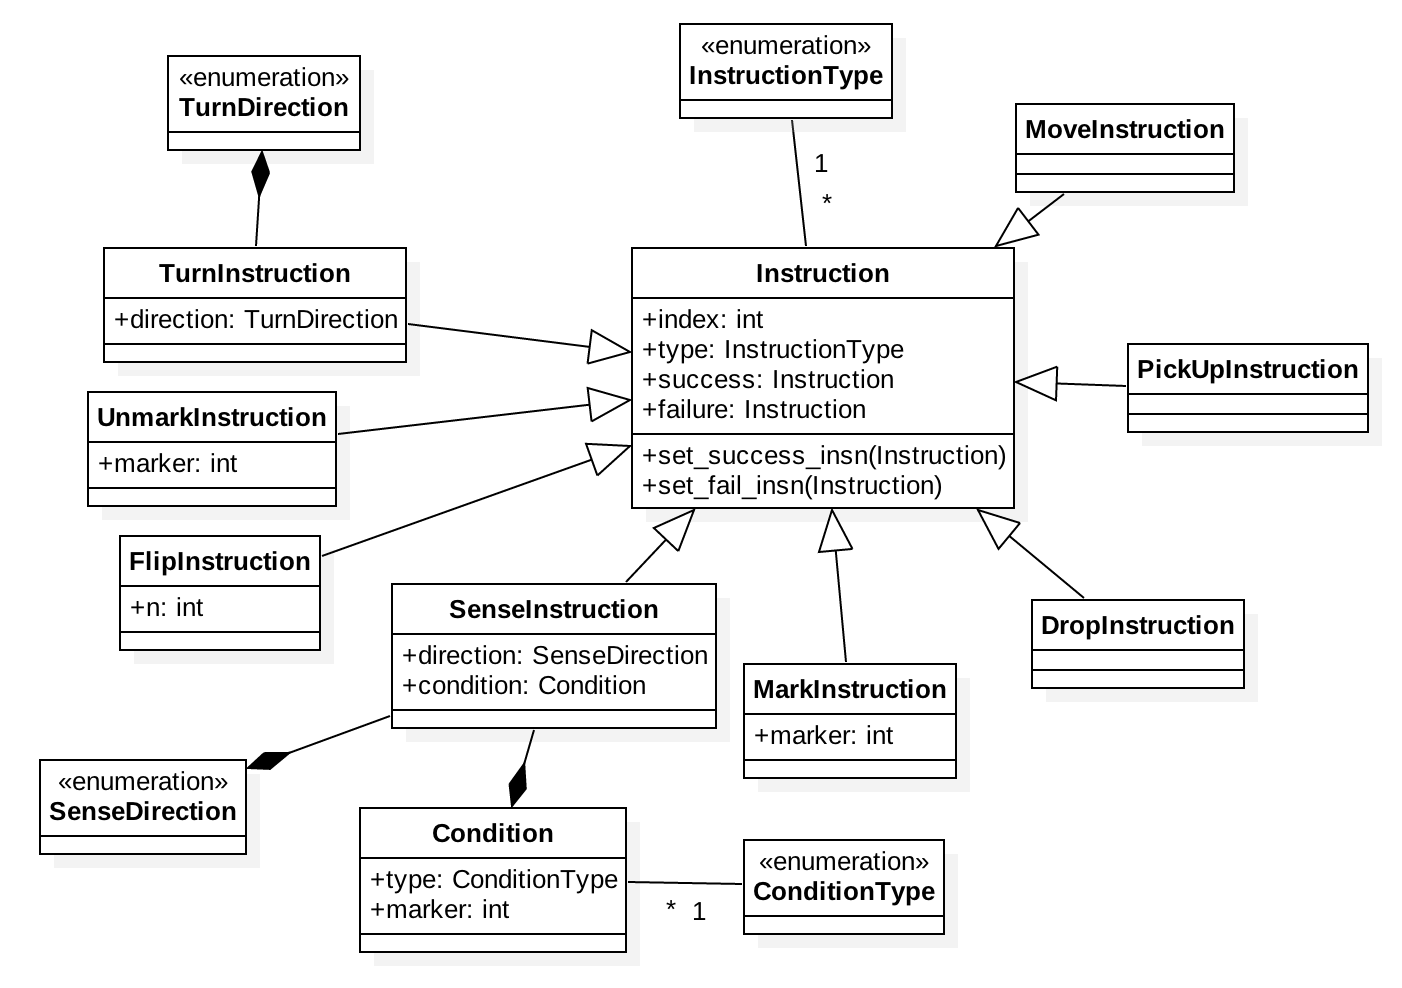
\includegraphics[width=0.8\textwidth]{low-level-diagrams/class/instruction.png}
\end{center}

\begin{longtable}[c]{@{}p{0.2\textwidth}p{0.7\textwidth}@{}}
\toprule
& Ant Game: Instructions\tabularnewline
\midrule

\texttt{TurnDirection} & An \texttt{enum} that describes the directions available for an ant to turn in - \texttt{left} or \texttt{right} as per functional requirement \texttt{Ant/6}. \tabularnewline
\texttt{TurnInstruction} & Represents an instruction that orders an ant to turn in a particular direction. The transition success state and fail state are both the same state. \tabularnewline
\texttt{UnmarkInstruction} & Represents an instruction that orders an ant to unmark a cell that holds a marker (of the same colony) of a given integer identifier. The transition success state and fail state are both the same state. \tabularnewline
\texttt{FlipInstruction} & Represents an instruction to generate a random number in the range \texttt{0..n}. \tabularnewline
\texttt{SenseDirection} & An \texttt{enum} that describes the directions available for an ant to sense in - \texttt{left-ahead}, \texttt{ahead}, and \texttt{right-ahead}. \tabularnewline
\texttt{Condition} & A class which represents a sense condition for an ant to validate on a cell. A condition has a type, and if it is a sense condition, also a marker identifier. \tabularnewline
\texttt{ConditionType} & An \texttt{enum} that represents possible conditions for an ant to check on a cell - see requirement \texttt{Ant/1}. \tabularnewline
\texttt{SenseInstruction} & A class which represents an order for an ant to check a condition on a cell in a specific direction. \tabularnewline
\texttt{MarkInstruction} & A class which represents an order for an ant to mark a cell. \textbf{Note}: the design specification for the \texttt{marker} field has been slightly modified - instead of an integer, the \texttt{MarkInstruction} class will use an instance of a \texttt{Marker} class, which holds an integer marker and \textit{also} an associated colony colour (red or black). \tabularnewline
\texttt{DropInstruction} & A class which represents an order for an ant to drop its food. The success and failure states for this class are the same state. \tabularnewline
\texttt{PickUpInstruction} & A class which represents an order for an ant to pick up the food on its current cell. \tabularnewline
\texttt{MoveInstruction} & A class which represents an order for an ant to step forward in its current direction. \tabularnewline
\texttt{InstructionType} & An enumeration which holds all possible instruction types - e.g. \texttt{DropInstruction}. \tabularnewline
\texttt{Instruction} & Finally, the abstract base class of all above instruction types --- this class stores information which is shared amongst its subclasses. Each instruction has an \texttt{index} (the line number, $0$-based), a type (holding the type of subclass), and two recursive instances of \texttt{Instruction} which hold the state to transition to if the ant's evaluation of this instruction is a success, and the state to transition to if the ant's evaluation of this instruction fails. For several subclasses, these are the same state. \tabularnewline
\bottomrule
\end{longtable}

\subsubsection{Brain}

Generating the above instruction data is done by the \textit{Brain Parser} component. As can be seen in the brain class diagram, a colony is composed of a colour and a brain - \textbf{note}: a colony of ants shares the same brain - an ant will, upon instantiation, get the start-instruction from the brain, and then keep track of its own state from then on. The brain parser exposes only one public method (to parse an ant brain file). The rest of the methods are to convert a string representation of the given type into the programmatic representation as per the instruction class diagram.

\begin{center}
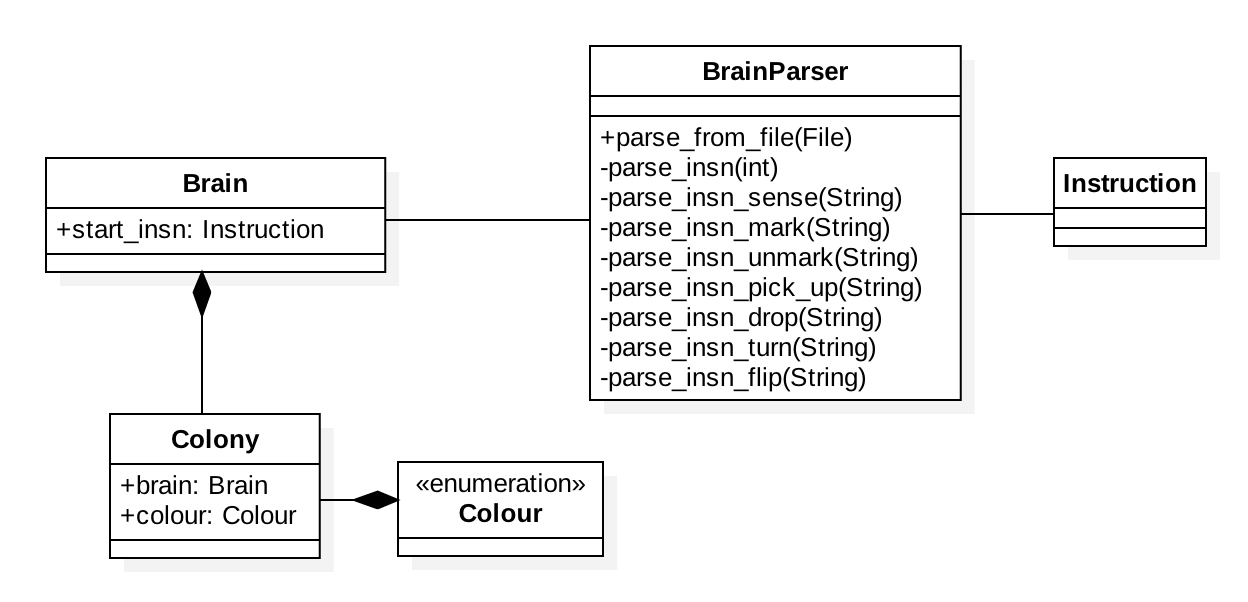
\includegraphics[width=0.8\textwidth]{low-level-diagrams/class/brain.png}
\end{center}

\begin{longtable}[c]{@{}p{0.2\textwidth}p{0.7\textwidth}@{}}
\toprule
& Ant Game: Brain\tabularnewline
\midrule

\texttt{Instruction} & This is a reference to the \texttt{Instruction} class in the previous diagram. \tabularnewline
\texttt{BrainParser} & This class has the purpose operation of translating a string-based representation of a brain graph constructed from the subclasses of \texttt{Instruction}. The \texttt{parse\_from\_file(File)} method should also validate the syntax of the brain specification. The internal design of the class is \textit{deliberately left unspecified}: it is left up to the programmers - either by stepping through the file line by line and connecting up the graph afterwards, or recursively parsing instructions based on the transition states that each line references. \tabularnewline
\texttt{Brain} & This class represents a unified brain of a colony. All ants share the same brain, but they do not share the same brain state - i.e. they keep track of the current state based on the return value of \texttt{Instruction\#success()}/\texttt{Instruction\#failure()}. \tabularnewline
\texttt{Colony} & As mentioned directly above, ants of the same colony share the same brain. So an instance of the brain is contained in the colony representation. A colony also has an associated colour, as below. \tabularnewline
\texttt{Colour} & Holds the possible colours of a colony - either red or black. \tabularnewline
\bottomrule
\end{longtable}

\subsubsection{World}

The next component of the system is the world-related content. The world parser reads a world specification from a file and produces a world instance. A world-generator instance can create a world instance via adding random contest-valid cells. A world is made up of an array of cells, which can have markers added and removed from them --- notice that a marker instance has an associated colony. In addition a cell can also hold an ant, which the world initialises via spawning the ants at the start of a game. 

\begin{center}
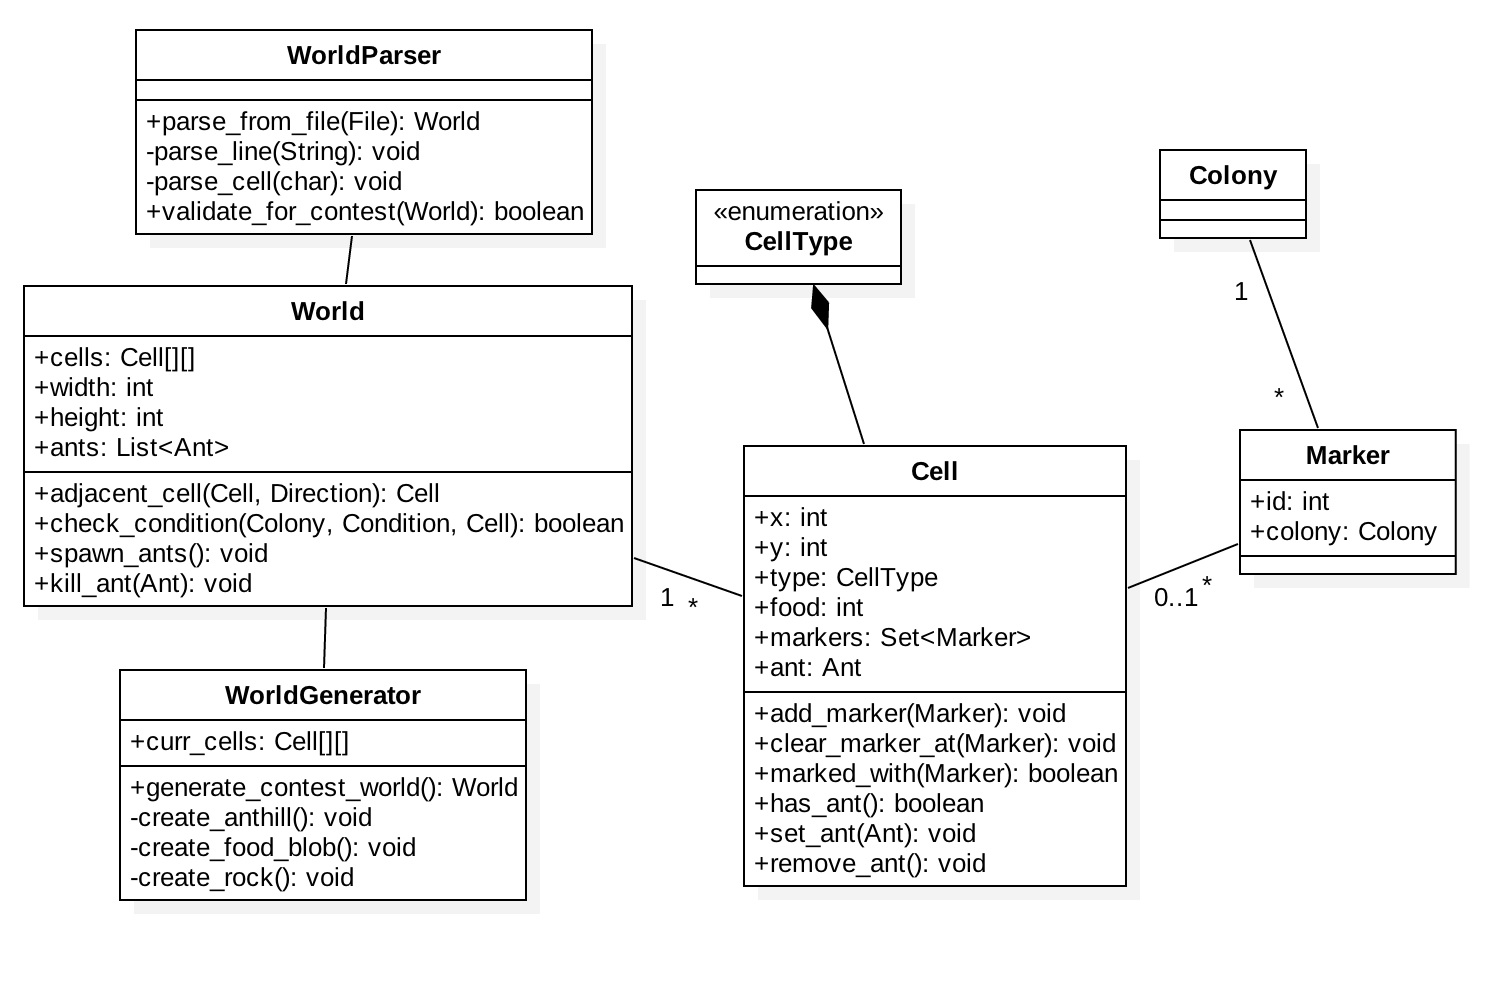
\includegraphics[width=0.8\textwidth]{low-level-diagrams/class/world.png}
\end{center}

\begin{longtable}[c]{@{}p{0.2\textwidth}p{0.7\textwidth}@{}}
\toprule
& Ant Game: World \tabularnewline
\midrule
\texttt{WorldParser} & Has the purpose of reading a world specification from a file. \textbf{Note}: additional operation requirement --- this class needs to expose a method \texttt{validate\_for\_contest(World)} which checks that a given world conforms to the tournament world specifications. \tabularnewline
\texttt{World} & Represents a game world and its associated state - that is, the world stores all cells and what they contain (food, markers, ants, rocks, \ldots) at any point. Exposes functionality to spawn and kill ants, check conditions on cells, find the adjacent hexagonal cell given a cell and direction. \tabularnewline
\texttt{WorldGenerator} & Used for generating random game worlds which conform to the tournament world specifications. \tabularnewline
\texttt{Cell} & The world is made up by a two-dimensional array of cells. Each cell contains information about what it holds - markers, ants, food particles. A cell instance exposes functionality for changing its state by adding and removing markers, ants, food. \tabularnewline
\texttt{CellType} & An enumerated type which holds all the different possible cells as per requirements - rock, clear, red anthill, black anthill. \tabularnewline
\texttt{Marker} & Notice that each marker holds not only the integer marker identifier, but also the associated colony - this is because cells store each colony's markers separately. \tabularnewline
\texttt{Colony} & As per previous table. \tabularnewline
\bottomrule
\end{longtable}

\subsubsection{Ant}

\begin{center}
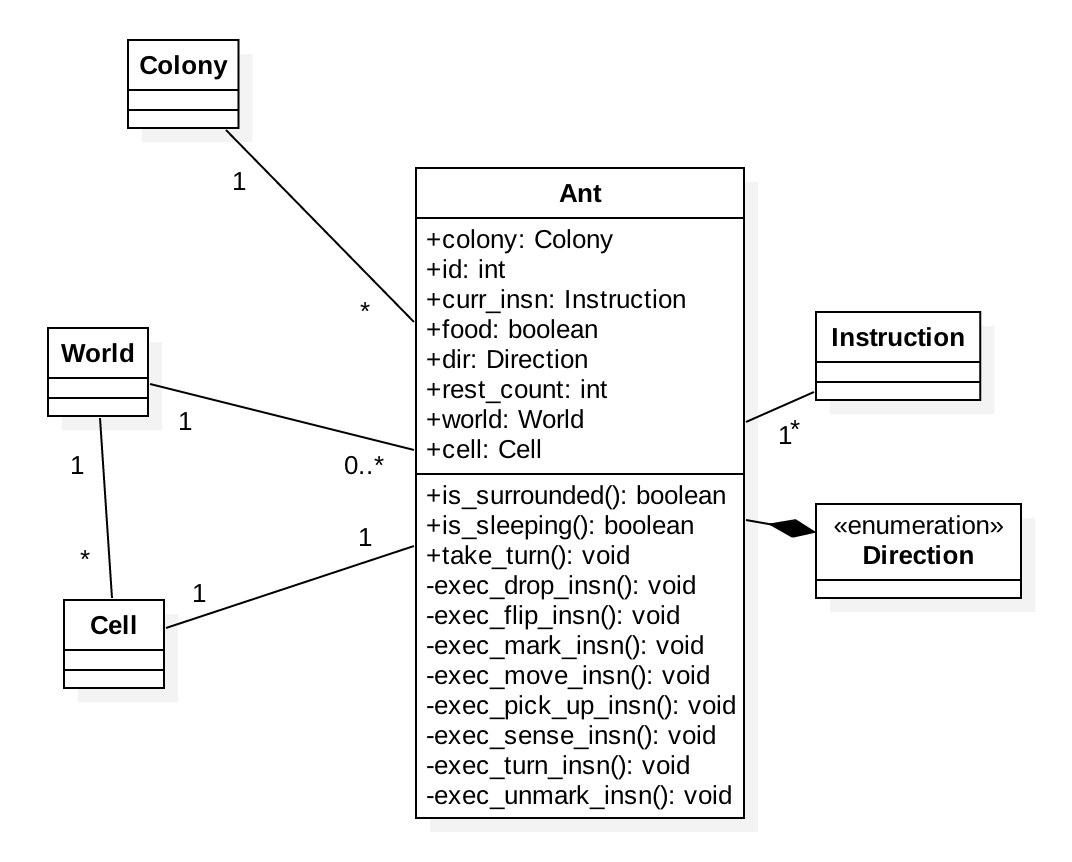
\includegraphics[width=0.8\textwidth]{low-level-diagrams/class/ant.png}
\end{center}

\begin{longtable}[c]{@{}p{0.2\textwidth}p{0.7\textwidth}@{}}
\toprule
& Ant Game: Ant \tabularnewline
\midrule
\texttt{Ant} & This is where the main logic for changing the state of the game world happens. An ant stores its own state (meaning the next instruction to execute on the world, as well as the unique ant identifier, the colony of the ant, whether the ant is holding food, the current direction in which it is facing, how many turns it is resting for --- 0 if not resting). It also has access to its current cell and also the world. The ant exposes functionality to check if it is surrounded by 5 or more foe ants, to test whether it is currently resting. Most importantly, it exposes the \texttt{take\_turn()} method, which executes an instruction. This method delegates to the relevant private method based on the instruction type. Each of these methods use the local state of the world to change the world's state, as well as the ants own state. \tabularnewline
\texttt{Direction} & This enumeration holds all possible hexagonal directions, as per the relevant section of the functional requirements. \tabularnewline
\bottomrule
\end{longtable}

\subsubsection{Game}

\begin{center}
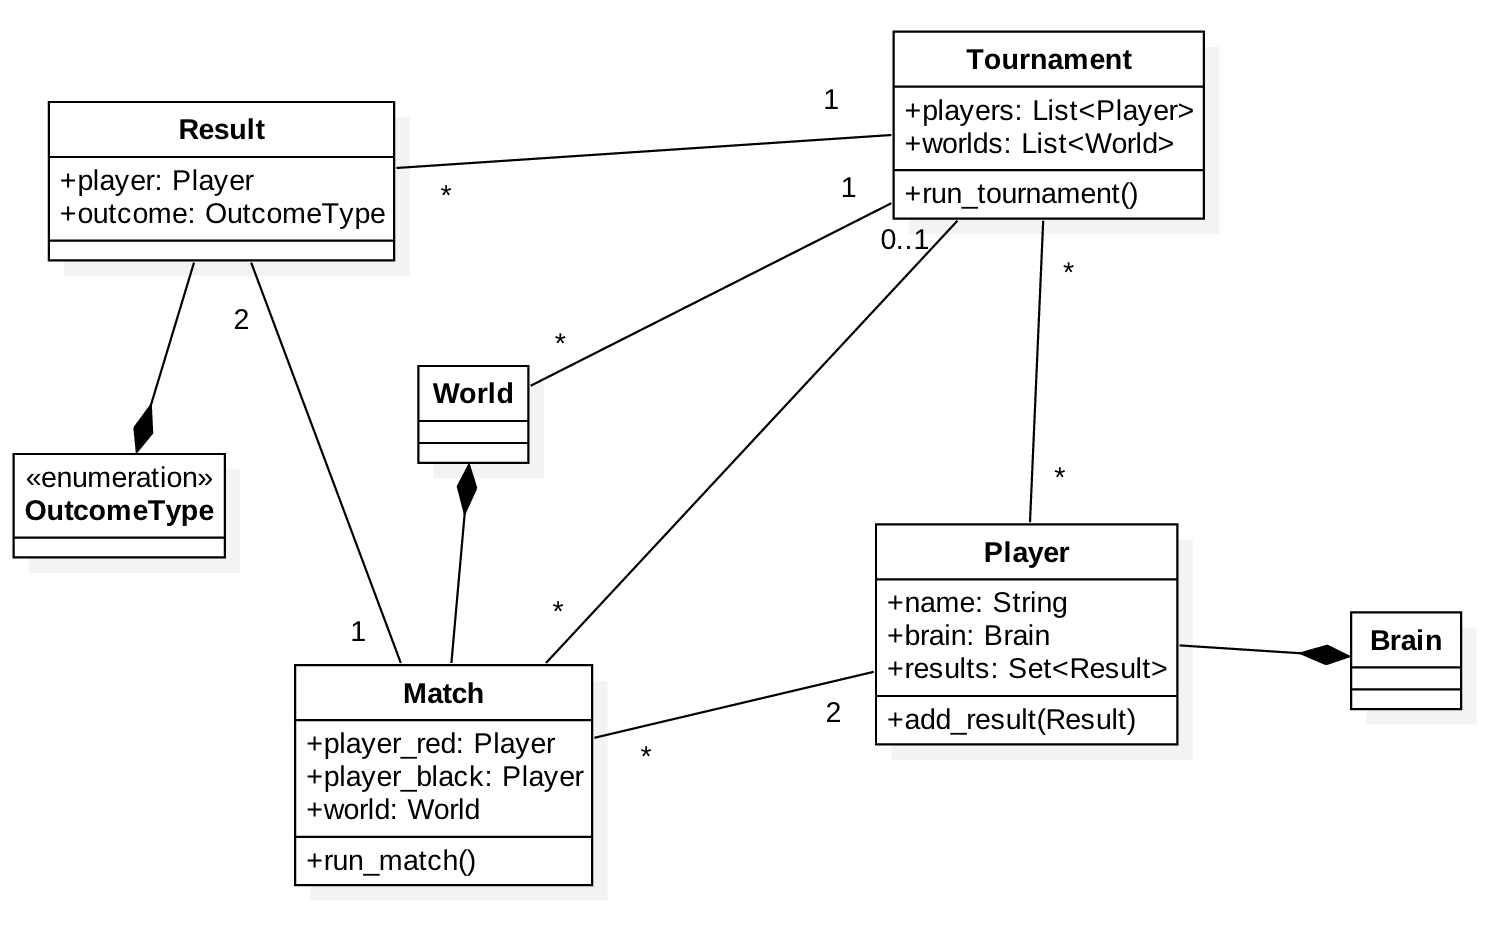
\includegraphics[width=0.8\textwidth]{low-level-diagrams/class/game.png}
\end{center}

\begin{longtable}[c]{@{}p{0.2\textwidth}p{0.7\textwidth}@{}}
\toprule
& Ant Game: Game \tabularnewline
\midrule
\texttt{Result} & A result is the outcome \textit{for a particular player} in a match. That is, for each result, there are three possible sets of two results: \{(player 1 win, player 2 loss), (player 2 win, player 1 loss), (player 1 draw, player 2 draw)\}. \tabularnewline
\texttt{OutcomeType} & The possible outcomes for a player in a match - win, loss, draw. \tabularnewline
\texttt{Match} & A match describes a pairing between two players on a world. One player is tied to the red colony of ants, and another player is tied to the black colony. The result of a match (\texttt{run\_match()}) is a set of two outcomes, one for each player. The job of the \texttt{run\_match()} method is to iterate 300,000 times over all the ants, making them take steps and then also checking to see whether the ants die from being surrounded. The ant colony with the most food in the anthill is then declared the winner. \tabularnewline
\texttt{Player} & A player essentially a programmatic model of an actual user. A user uploads an ant brain from the interface, and specifies a team name. They then can compete in either a tournament or a match. A player maintains a set of results, possibly from a single match or a tournament. \tabularnewline
\texttt{Tournament} & A tournament can be treated as a collection of all possible matches as per functional requirements (see \texttt{Game/3}). The tournament simply creates matches between the players, and then executes them. Score counting is done as per requirement \texttt{Game/3}, and so is team elimination if drawing occurs. \tabularnewline
\bottomrule
\end{longtable}

\textbf{Note}: further to the above, an additional integration of the game with the world must be added to the current design. As per requirement \texttt{Game/2}, statistics must be produced for a game. This involves:
\begin{itemize}
\item integrating statistics tracking into the \texttt{Match\#run\_match()} method --- by examining the state changes occurring to the world after each match iteration, increment relevant local variables to track the statistics specified in \texttt{Game/2}.
\item the tournament statistics should track the \textit{total} statistics over all games.
\item these statistics should be accessible (by return value) to the interface. 
\end{itemize}

\subsection{Interface}

The interface design is left up to the discretion of the programmers, however the properties of the interface are shown in this section. The interface will be composed of several `screens', detailed on the following pages.

\subsubsection{Start Screen}

\begin{center}
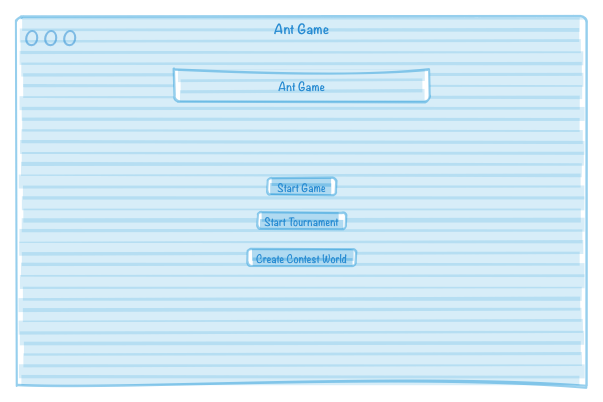
\includegraphics[width=\textwidth]{low-level-diagrams/interface/start-screen}
\end{center}

\begin{itemize}
\item The \texttt{Start Game} button will switch the screen to the game setup screen.
\item The \texttt{Start Tournament} button will switch the screen to the tournament setup screen.
\item The \texttt{Create Contest World} button will generate a random valid contest world and save it to file, using a file chooser dialog to let the user choose the save location and name.
\end{itemize}

\subsubsection{Game Setup Screen}

\begin{center}
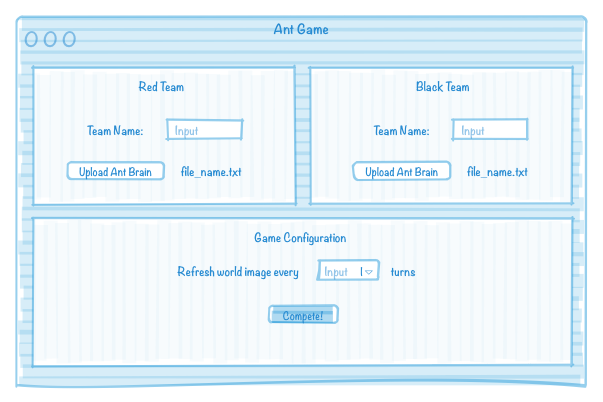
\includegraphics[width=\textwidth]{low-level-diagrams/interface/game-setup-screen}
\end{center}

\begin{itemize}
\item The teams should be able to input a name into the text input boxes, which should set the team name.
\item The teams should be able to click the \texttt{Upload Ant Brain} button --- at which point a file chooser dialog should pop up, allowing the user to select their ant brain. Upon selection, the ant brain should be parsed --- if failed, the parsing error message should be shown to the user.
\item The input at the bottom is for the user to set how often the world view should refresh on the GUI (an integer).
\item Upon clicking the `Compete!' button, the screen should transition to the game screen. 
\end{itemize}

\subsubsection{Game Screen}

\begin{center}
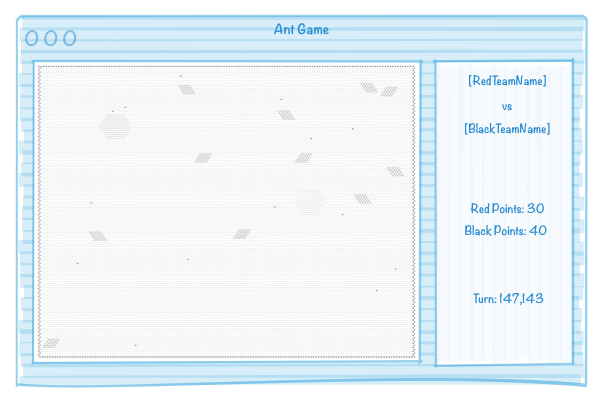
\includegraphics[width=\textwidth]{low-level-diagrams/interface/game-screen}
\end{center}

\begin{itemize}
\item The game screen shall show the state of the game world (differentiating between ants, food cells, obstacles, anthills) every \texttt{n} turns as specified in the previous screen.
\item The turn number and team points (food in anthills) are shown on the right, along with the player names.
\end{itemize}

\subsubsection{Game Statistics Screen}

\begin{center}
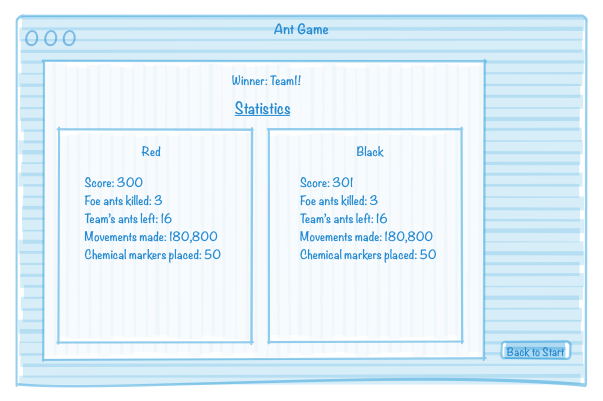
\includegraphics[width=\textwidth]{low-level-diagrams/interface/game-statistics-screen}
\end{center}

\begin{itemize}
\item The winner of the match should be displayed at the top. If it is a draw, it will say `Draw!' instead.
\item Each statistics view for each team will contain all of the statistics required from the functional requirements.
\item The button in the bottom right will bring the user back to the start screen.
\end{itemize}

\subsubsection{Tournament Setup Screen}

\begin{center}
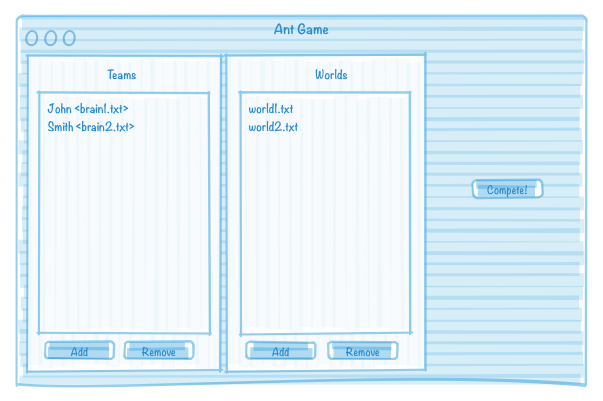
\includegraphics[width=\textwidth]{low-level-diagrams/interface/tournament-setup-screen}
\end{center}

\begin{itemize}
\item Teams can be added and removed from a list. When the \texttt{Add} button is clicked, an input dialog pops up asking for a user's name. Then a file chooser pops up asking for the user's ant brain file. The file is parsed - as always, if a parsing error occurs it is displayed to the user. A string representation of the team is added to the list.
\item The remove button removes a team from the list.
\item The world list behaves identically, except no name dialog appears.
\item The \texttt{Complete} dialog transitions the screen to the tournament screen.
\end{itemize}

\subsubsection{Tournament Screen}

\begin{itemize}
\item The tournament screen is the same as the two-player game screen, except that after each game the screen transitions to the game screen for the next match.
\end{itemize}

\subsubsection{Tournament Statistics Screen}

\begin{center}
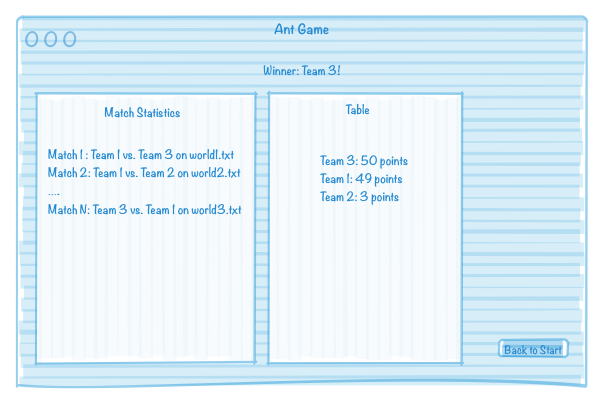
\includegraphics[width=\textwidth]{low-level-diagrams/interface/tournament-statistics-screen}
\end{center}

\begin{itemize}
\item The left panel is a listing of all matches, in order of execution. Upon double-clicking a mini-dialog pops up showing the statistics for that game (identically to the game statistics panel).
\item The score table on the right is a listing of the team and their points, in descending order.
\item The header at the top is the winner of the tournament.
\item The button in the bottom right is takes the user back to the start screen.
\end{itemize}

\end{document}
